\documentclass [11pt]{book}

\author {Dave Cooper}

\textwidth 6.5in

\topmargin 0in

\textheight 8.5in

\oddsidemargin 0in

\evensidemargin 0in

\pdfimageresolution 135

\title {GenDL Unified Documentation}

\usepackage [dvips]{graphicx}

\usepackage [usenames, dvipsnames]{color}

\usepackage {makeidx}

\usepackage {textcomp}

\usepackage [colorlinks=true, urlcolor=cyan]{hyperref}

\newsavebox {\boxedverb}

\makeindex 



\begin{document}



\frontmatter



\maketitle


\footnotetext{Copyright 
\copyright{} 2012, Genworks International. Duplication, by any means, in whole or in part, requires 
written consent from Genworks International.}

\tableofcontents



\mainmatter



\chapter{Introduction}

\label{chap:introduction}



\section{Welcome}

\label{sec:welcome}

Congratulations on your purchase or download of Genworks Gendl. By investing some of your 
valuable time into learning this system, you are investing in your future productivity and you are becoming
part of a quiet revolution. Although you may have come to Genworks Gendl because of an interest in 3D modeling
or mechanical engineering, you will find that a whole new world, and a whole new approach to computing, will 
now be at your fingertips.

\section{Knowledge Base Concepts According to Genworks}

\label{sec:knowledgebaseconceptsaccordingtogenworks}

You may have an idea about Knowledge Base Systems,
or Knowledge \emph{Based} Systems, from college textbooks or corporate marketing propaganda, and found the 
concept too broad to be of practical use. Or you may have heard jabs at the 
pretentious-sounding name, ``Knowledge-based Engineering,'' as in: ``you mean as opposed to \index{Ignorance-based Engineering}Ignorance-based Engineering?'' 

To provide a clearer picture, we hope you will agree that our concept
of a KB system is simple and practical, and in this tutorial our goal
is to make you comfortable and excited about the ideas we have
implemented in our flagship system, GenDL (or ``Gendl'' 


Our definition of a \emph{\index{Knowledge Base System}Knowledge Base System} is an object-oriented programming environment which implements the features of \emph{\index{Caching}Caching} and \emph{\index{Dependency tracking}Dependency tracking}. Caching means that once the KB has computed something, it might not need to repeat 
that computation if the same question is asked again. Dependency tracking is the flip side
of that coin --- it ensures that if a cached result is \emph{stale}, the result will be recomputed the next time it is \emph{demanded}, so as to give a fresh result.

\section{Goals for this Tutorial}

\label{sec:goalsforthistutorial}

This manual is designed as a companion to a live two-hour GDL/GWL tutorial, but you may
also be reading it on your own. In either case, the basic goals are:

\begin{itemize}

\item Get you excited about using GDL/GWL

\item Enable you to judge whether GDL/GWL is an appropriate tool for a given job

\item Arm you with the ability to argue the case for using GDL/GWL when appropriate

\item Prepare you to begin maintaining and authoring GDL/GWL applications, or porting apps
from similar KB systems into GDL/GWL.

\end{itemize}

This manual will begin with an introduction to the \index{Common Lisp}Common Lisp programming language. If you are new to Common Lisp:
congratulations! You have just discovered a powerful tool backed by a
powerful standard specification, which will protect your development
investment for decades to come. In addition to the brief overview in
this manual, many resources are available to get you started in CL ---
for starters, we recommend 
\underline{\index{Basic Lisp Techniques}Basic Lisp Techniques}\footnote{
\underline{BLT} is available at \texttt{http://www.franz.com/resources/educational\_resources/cooper.book.pdf}}, which was prepared by the author of this tutorial. 

\section{What is GenDL?}

\label{sec:whatisgendl?}

GenDL (or Gendl to be a bit more relaxed) is an acronym for
``General-purpose Declarative Language.'' 

GenDL is a superset of ANSI Common Lisp, and consists mainly of
automatic code-expanding extensions to Common Lisp implemented in the
form of macros. When you write, let's say, 20 lines in GenDL, you
might be writing the equivalent of 200 lines of Common Lisp. Of
course, since GenDL is a superset of Common Lisp, you still have the
full power of the CL language at your fingertips whenever you are
working in GenDL.

\index{compiled language!benefits of}\index{macros!code-expanding}Since GDL expands into CL, everything you write in GDL will be
compiled ``down to the metal'' to machine code with all the
optimizations and safety that the tested-and-true CL compiler
provides. This is an important distinction as contrasted to some other
so-called KB systems on the market, which are really nothing more than
interpreted scripting languages which often impose arbitrary limits on
the size and complexity of your application.

GenDL is also a true \emph{\index{declarative}declarative} language. When you put together a GDL application, you write and think mainly
in terms of objects and their properties, and how they depend on one another in a direct
sense. You do not have to track in your mind explicitly how one object or property will ``call''
another object or propery, in what order this will happen, etc. Those details are
taken care of for you automatically by the language. 

Because GDL is object-oriented, you have all the features you would normally expect
from an object-oriented language, such as 

\begin{itemize}

\item Separation between the \emph{definition} of an object and an \emph{instance} of an object

\item High levels of data abstraction

\item The ability for one object to ``inherit'' from others

\item The ability to ``use'' an object without concern for its ``under-the-hood'' implementation

\end{itemize}

\index{object-orientation!message-passing}\index{object-orientation!generic-function}GDL supports the ``message-passing'' paradigm of object orientation, with some extensions. Since
full-blown ANSI CLOS (Common Lisp Object System) is always available as well, the Generic Function paradigm 
is supported as well. Do not be concerned at this point if you are not fully aware of the differences 
between these two paradigms\footnote{See Paul Graham's 
\underline{ANSI Common Lisp}, page 192, for an excellent discussion of the Two Models 
of Object-oriented Programming.}.

\section{Why GDL (what is GDL good for?)}

\label{sec:whygdl(whatisgdlgoodfor?)}



\begin{itemize}

\item Organizing and interrelating large amounts of information
in ways not possible or not practical using conventional languages or 
conventional relational database technology alone;

\item Evaluating many design or engineering alternatives and 
performing various kinds of optimizations within specified design
spaces;

\item Capturing the procedures and rules used to solve repetitive
tasks in engineering and other fields;

\item Applying rules to achieve intermediate and final 
outputs, which may include virtual models of wireframe, surface,
and solid geometric objects.

\end{itemize}



\section{What GDL is not}

\label{sec:whatgdlisnot}



\begin{itemize}

\item A CAD system (although it may operate on and/or generate geometric entities);

\item A drawing program (although it may operate on and/or generate geometric entities);

\item An Artificial Intelligence system (although it is an excellent environment for developing 
capabilities which could be considered as such);

\item An Expert System Shell (although one could be easily embedded within it).

\end{itemize}

Without further ado, then, let's turn the page and get started with some hands-on GDL...

\chapter{Installation}

\label{chap:installation}

Follow Section 
\ref{sec:installationofpre-packagedgendl} if your email address is registered with Genworks and you will
install a pre-packaged Gendl distribution including its own Common
Lisp engine.  Gendl is also available as open-source software\footnote{http://github.com/genworks/Genworks-GDL}; if you
want to use that version, then please refer to Section 
\ref{sec:installationofopen-sourcegendl}.

\section{Installation of pre-packaged Gendl}

\label{sec:installationofpre-packagedgendl}

This section will take you through the installation of Gendl
from a prepackaged distribution with the Allegro CL Common Lisp engine
and the Slime IDE (based on Gnu Emacs).

\subsection{Download the Software and retrieve a license key}

\label{subsec:downloadthesoftwareandretrievealicensekey}



\begin{enumerate}

\item Visit the Downloads section of the \href{http://genworks.com/newsite}{Genworks Newsite}

\item Enter your email address\footnote{if your address is not on file, send mail to licensing@genworks.com}.

\item Download the latest Payload and gpl.zip for Windows\footnote{If you already have a gpl.zip from a previous Gendl installation, it is not necessary to download a new one.}

\item Click to receive license key file by email.

\end{enumerate}



\subsection{Unpack the Distribution}

\label{subsec:unpackthedistribution}

GenDL is currently distributed for all the platforms as a
self-contained ``zip'' file which does not require official
administrator installation.  What follows are general instructions; more up-to-date details
may be found in the email which accompanies the license key file. A five-minute installation video
is also available in the Documentation section of the \href{http://genworks.com/newsite}{Genworks Newsite}.

\begin{enumerate}

\item Unzip the gdl1581... zipfile into a location where you have write permissions

\item Unzip the gpl.zip file at the same level as the gdl payload

\item Copy the license key file as gdl.lic (for Trial,
	 Student, Professional editions), or devel.lic (for Enterprise edition) into the \texttt{program/} directory within the gdl1581.../ directory.

\end{enumerate}


\begin{figure}
\begin{center}
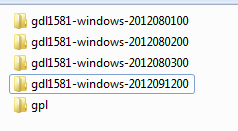
\includegraphics{../images/gendl-installation.png}
\end{center}

\caption{Several Gendl versions and one GPL }

\label{fig:gendl-installation}

\end{figure}
So you now should have two directories at the same level: one named \texttt{gdl1581.../}(the rest of the name will contain the specific dated build stamp), and a \texttt{gdl/}directory at the same level. Note that as seen in Figure 
\ref{fig:gendl-installation}, it is possible to have several Gendl versions installed, but just a single common \texttt{gpl/} folder.

\subsection{Make a Desktop Shortcut}

\label{subsec:makeadesktopshortcut}



\begin{enumerate}

\item Using the ``My Computer'' or ``Computer'' Windows file manager, right-mouse on the \texttt{run-gdl.bat} file.

\item Select ``Create Shortcut.''

\item Now drag the new ``Run-gdl-shortcut'' icon to your desktop.

\end{enumerate}



\subsection{Populate your Initialization File}

\label{subsec:populateyourinitializationfile}

The default initialization file for Gendl is called \texttt{gdlinit.cl}, 

\section{Installation of open-source Gendl}

\label{sec:installationofopen-sourcegendl}

This section is only relevant if you have not received a
pre-packaged Gendl distribution with its own Common Lisp engine.  If
you have received a pre-packaged Gendl distribution, then please skip
this section. In case you want to use the open-source Gendl, you will
use your own Common Lisp installation and fetch Gendl (Genworks-GDL)
using a very powerful and convenient CL package/library manager
called \emph{Quicklisp}.

\subsection{Install and Configure your Common Lisp environment}

\label{subsec:installandconfigureyourcommonlispenvironment}

Gendl is currently tested to build on the following Common Lisp engines:

\begin{itemize}

\item Allegro CL (commercial product from Franz Inc, free Express Edition available)

\item LispWorks (commercial product from LispWorks Ltd, free Personal Edition available)

\item Steel Bank Common Lisp (SBCL) (free open-source project with permissive license)

\end{itemize}

Please refer to the documentation for each of these systems for full information on installing 
and configuring the environment. Typically this will include a text editor, either Gnu Emacs with Superior
Lisp Interaction Mode for Emacs (Slime), or a built-in text editing and development environment which 
comes with the Common Lisp system.

As of this writing, a convenient way to set up Emacs with Slime is to use the \href{http://github.com/quicklisp/quicklisp-slime-helper}{Quicklisp-slime-helper}.

\subsection{Load and Configure Quicklisp}

\label{subsec:loadandconfigurequicklisp}

As of this writing, Quicklisp is rapidly becoming the defacto standard library manager for Common Lisp.

\begin{itemize}

\item Visit the \href{http://quicklisp.org}{Quicklisp website}

\item Follow the instructions there to download the \texttt{quicklisp.lisp} bootstrap file and load it to set up your Quicklisp environment.

\end{itemize}



\section{System Startup and Testing}

\label{sec:systemstartupandtesting}



\subsection{System Startup}

\label{subsec:systemstartup}



\subsubsection{Startup of prepackaged Gendl distribution}

\label{subsubsec:startupofprepackagedgendldistribution}

To start a prepackaged system, follow these steps:

\begin{enumerate}

\item Invoke the \texttt{run-gdl.bat} (Windows), or \texttt{run-gdl} (Linux, MacOS) startup script. This should launch Gnu Emacs with a 
README file displayed by default. Take the time to look through this README file. 
Especially the later part of the file contains information about Emacs keyboard
shortcuts available.

\item In emacs, enter: \texttt{M-x glime}. That is, hold down the ``Meta'' (or ``Alt'') key, and press the ``X'' key, then type ``glime.''
You will see this command shown in the \emph{mini-buffer} at the bottom of the Emacs window, as shown in Figure 
\ref{fig:mini-buffer}

\begin{figure}
\begin{center}
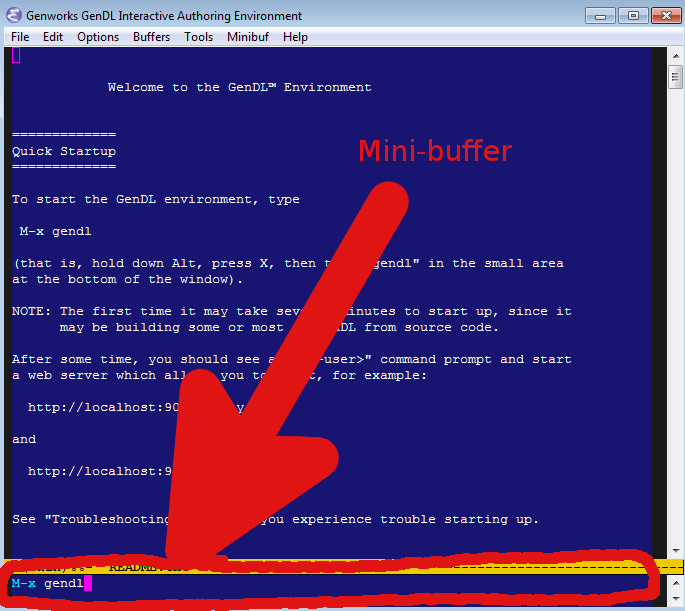
\includegraphics[width=3in,height=3in]{../images/mini-buffer.png}
\end{center}

\caption{The mini-buffer in Emacs}

\label{fig:mini-buffer}

\end{figure}

\item press the ``Enter'' key

\begin{figure}
\begin{center}
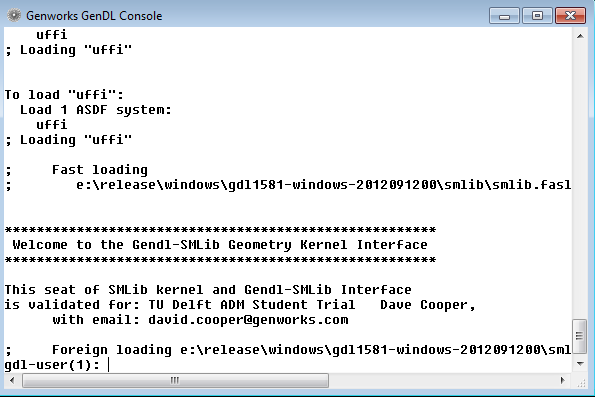
\includegraphics{../images/genworks-gendl-console.png}
\end{center}

\caption{Genworks Gendl Console}

\label{fig:genworks-gendl-console}

\end{figure}

\item On Windows, you will get a new window, named the the \index{Genworks Gendl Console}Genworks Gendl Console, as shown in Figure 
\ref{fig:genworks-gendl-console}. This window might start out in minimized form (as an icon at the bottom of your screen). Click on it 
to open it. Watch this console for any errors or warnings. 

The first time you start up, you may see messages in this console for
several minutes while the system is being built (or if you received a
completely pre-built system, the messages may last only a few
seconds).

On Linux or MacOS, there will be a separate Emacs buffer (available
through Emacs' ``Buffers'' menu) where you will see these messages.

The messages will consist of compiling and loading information, followed by copyright and welcome information
for Gendl. After these messages have finished, you should see the following command prompt:

\texttt{\index{gdl-user(1): }gdl-user(1): }

The Genworks GenDL console contains a command prompt, but mostly you will use the \index{*slime-repl...*}*slime-repl...* buffer in Emacs to type commands. The Genworks GenDL console is mainly used for 
displaying output text from the Gendl system and from your application.

\end{enumerate}



\subsubsection{Startup of open-source Gendl distribution}

\label{subsubsec:startupofopen-sourcegendldistribution}

To start an Open-source distribution, follow these steps:

\begin{enumerate}

\item Start your Common Lisp engine and development environment (e.g. SBCL with Emacs and Superior Lisp Interaction Mode for Emacs).

\item After Quicklisp is installed and initialized in your system, type: \texttt{(ql:quickload :genworks-gdl)} to get Genworks Gendl installed and loaded in your environment.

\item Type the following to initialize the Gendl environment:

\texttt{(gdl:start-gdl :edition :open-source)}



\end{enumerate}



\subsection{Basic System Test}

\label{subsec:basicsystemtest}

You may test your installation using the following
checklist. These tests are optional. You may perform some or all of
them in order to ensure that your Gendl is installed correctly and
running smoothly. In your Web Browser (e.g. Google Chrome, Firefox,
Safari, Opera, Internet Explorer), perform the following steps:

\begin{enumerate}

\item visit http://localhost:9000/tasty.

\item accept default robot:assembly.

\item Select ``Add Leaves'' from the Tree menu.

\item Click on the top node in the tree.

\item Observe the wireframe graphics for the robot as shown in 
\ref{fig:tasty-robot}.

\begin{figure}
\begin{center}
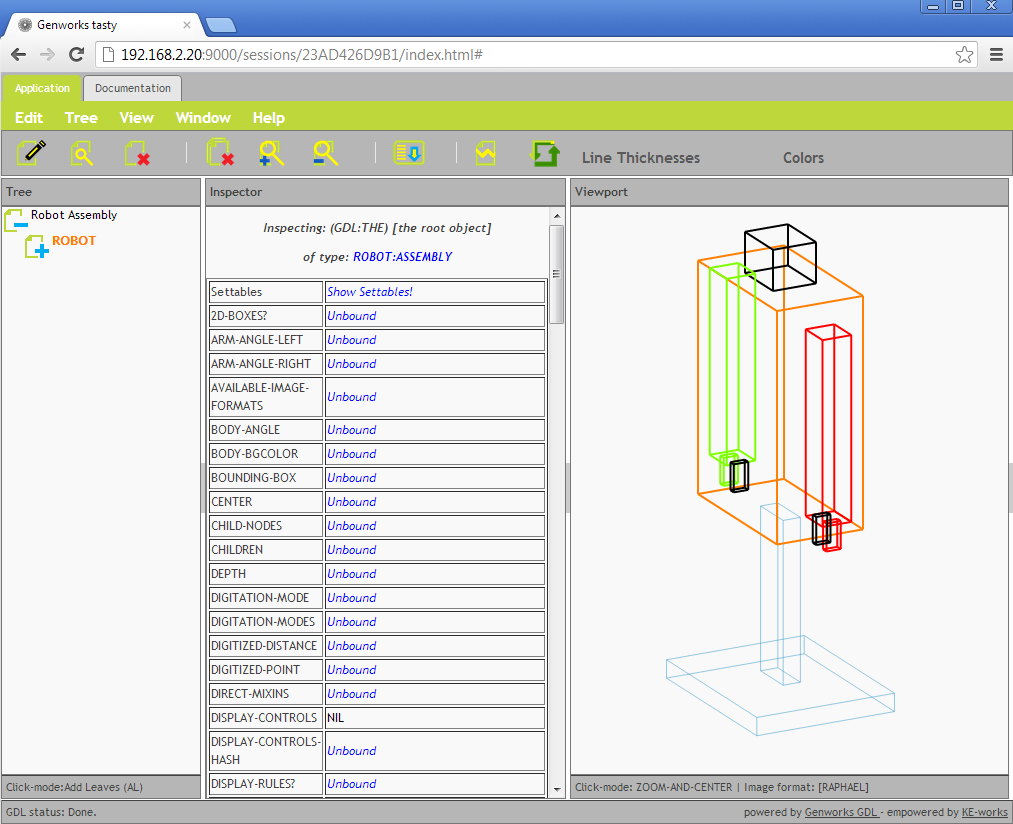
\includegraphics[width=3in,height=3in]{../images/tasty-robot.png}
\end{center}

\caption{Robot displayed in Tasty}

\label{fig:tasty-robot}

\end{figure}

\begin{figure}
\begin{center}
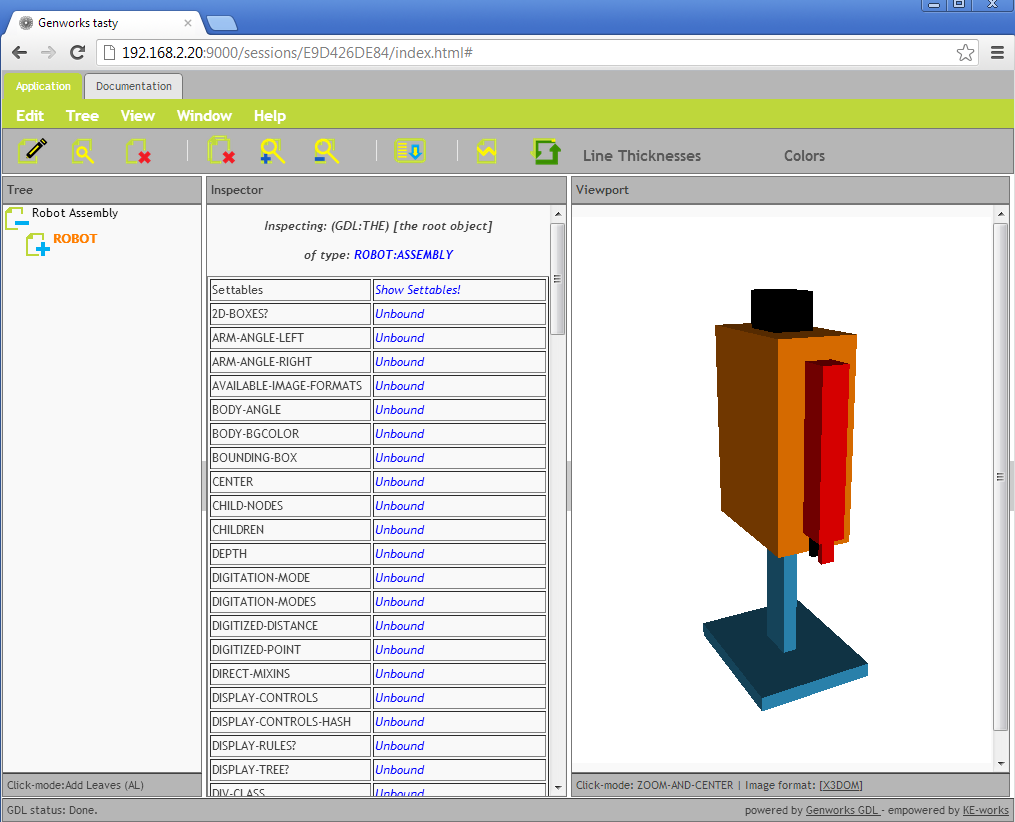
\includegraphics[width=3in,height=3in]{../images/tasty-robot-x3dom.png}
\end{center}

\caption{Robot x3dom}

\label{fig:tasty-robot-x3dom}

\end{figure}

\item Click on the robot to zoom in.

\item Select ``Clear View!'' from the View menu.

\item Select ``X3DOM'' from the View menu.

\item Click on the top node in the tree.

\item ``Refresh'' or ``Reload'' your browser window (may not be necessary).

\item If your browser supports WebGL, you will see the robot in shaded dynamic view as shown in Figure
\ref{fig:tasty-robot-x3dom}.

\item Select ``PNG'' from the View menu. You will see the wireframe view of the robot as a PNG image.

\item Select ``X3D'' from the View menu. If your browser has an X3D plugin installed (e.g. BS Contact), 
you will see the robot in a shaded dynamic view.

\end{enumerate}



\subsection{Full Regression Test}

\label{subsec:fullregressiontest}

\index{regression tests}The following commands will invoke a full regression test, including a test of the Surface and Solids
primitives provided by the SMLib geometry kernel. Note that the SMLib geometry kernel is only available with
proprietary Gendl licenses --- therefore if you have an open-source or Trial version, you these regression
tests will not all function.

In Emacs at the \texttt{gdl-user>} prompt in the \texttt{*slime-repl...*} buffer, type the following commands:

\begin{enumerate}

\item \texttt{(ql:quickload :gdl-regression)}

\item \texttt{(gdl-lift-utils::define-regression-tests)}

\item \texttt{(gdl-lift-utils::run-regression-tests-pass-fail)}

\item \texttt{(pprint gdl-lift-utils::*regression-test-report*)}

\end{enumerate}



\section{Getting Help and Support}

\label{sec:gettinghelpandsupport}

If you run into unexplained errors in the installation and startup process, please contact the following resources:

\begin{enumerate}

\item Make a posting to the \href{http://groups.google.com/group/genworks}{Genworks Google Group}

\item For pure Common Lisp issues, join the \#lisp IRC (Internet Relay Chat) channel and discuss issues there.

\item Also for Common Lisp issues, follow the comp.lang.lisp Usenet group.

\item If you are a supported Genworks customer, send email to \href{mailto:support@genworks.com}{support@genworks.com}

\item If you are not a supported Genworks customer but you want to report an apparent bug or have other suggestions or inquiries, you may also send email to \href{mailto:support@genworks.com}{support@genworks.com}, but please understand that Genworks cannot guarantee any response or a particular timeframe for any response.

\end{enumerate}



\chapter{Basic Operation of the Gendl Environment}

\label{chap:basicoperationofthegendlenvironment}

This chapter will step you through all the basic steps of
operating a typical Gendl environment. We will not go into any depth
about the additional features of the environment or language syntax in
this section --- this is just for getting familiar and practicing with
the mechanics of operating the environment with a keyboard.

\section{What is Different about Gendl?}

\label{sec:whatisdifferentaboutgendl?}

Gendl is  a dynamic language environment with incremental compiling and in-memory 
definitions. That means that as long as the system is running, you can \emph{compile} new \emph{definitions} of functions, objects, etc, and they will immediately become available as part of the running system,
and you can begin testing them immediately or update an existing set of objects to observe their new behavior.

In many other programming language systems, you have to start the
system from the beginning and reload all the files in order to test
new functionality. 
 
In Gendl, if you simply shut down the system after having compiled and
loaded a set of files with new definitions, then when you restart the
system you will have to recompile and/or reload those definitions in
order to bring the system back into the same state. This is typically
done automatically, using commands placed into the \texttt{gdlinit.cl} initialization file, as introduced in Section 
\ref{sec:customizingyourenvironment}. Alternatively, you can compile and load definitions into your Gendl
session, then save the ``world'' in that state. That way, it is
possible to start a new Gendl ``world'' which already has all your
application's definitions loaded and ready for use, without having to
procedurally reload any files. You can then begin to make and test new
definitions (and re-definitions) starting from this new ``world.''

\section{Startup, ``Hello, World!'' and Shutdown}

\label{sec:startup,hello,world!andshutdown}



The typical Gendl environment consists of three programs: Gnu
Emacs (the editor), a Common Lisp engine with Gendl system loaded or built into it (e.g. the \texttt{gdl.exe} executable in your \texttt{program/} directory), and (optionally) a web browser
such as Firefox, Google Chrome, Safari, Opera, or Internet
Explorer. Emacs runs as the main \emph{process}, and this in turn starts the CL engine with Gendl as a \emph{sub-process}. The CL engine typically runs an embedded \emph{webserver}, enabling you to access your application through a standard web browser.



As introduced in Chapter 
\ref{chap:installation}, the typical way to start a pre-packaged Gendl environment is with the \texttt{run-gdl.bat} (Windows), or \texttt{run-gdl} (MacOS, Linux) script files. Invoke this script file
from your computer's file manager, or from a desktop shortcut if you
have created one as outlined in section 
\ref{subsec:makeadesktopshortcut}. Your installation executable may also have created a
Windows ``Start'' menu item for Genworks Gendl. Of course you can also 
invoke \texttt{run-gdl.bat} from the Windows ``cmd'' command-line, or from another command shell such as Cygwin.\footnote{Cygwin is also useful as a command-line tool on Windows
for interacting with a version control system like Subversion (svn).}



\subsection{Startup}

\label{subsec:startup}

 Startup of a typical Gendl development session consists of
two fundamental steps: (1) starting the Emacs editing environment,
and (2) starting the actual Gendl process as a ``sub-process'' or ``inferior'' process 
within Emacs. The Gendl process should automatically establish a network connection
back to Emacs, allowing you to interact directly with the Gendl process from within Emacs.

\begin{enumerate}

\item Invoke the \texttt{run-gdl.bat} or \texttt{run-gdl.bat} startup script.

\item You should see a blue emacs window as in Figure 
\ref{fig:emacs-startup}. (alternative colors are also possible).

\item Press M-x (Alt-x), and type \texttt{gendl} in the mini-buffer, as seen in Figure 
\ref{fig:mini-buffer}.

\item (MS Windows): Look for the Genworks Gendl Console
window, or (Linux, Mac) use the Emacs ``Buffer'' menu to visit the
``*inferior-lisp*'' buffer. Note that the Genworks Gendl Console
window might start as a minimized icon; click or double-click it to
un-minimize.

\item Watch the Genworks GDL Console window for any
errors. Depending on your specific installation, it may take from a
few seconds to several minutes for the Genworks Gendl Console (or
*inferior-lisp* buffer) to settle down and give you a \texttt{gdl-user(): } prompt. This window is where you will see most of your program's textual output, any 
error messages, warnings, etc.

\item In Emacs, type: \texttt{C-x \&} (or select Emacs menu item Buffers$\rightarrow$*slime-repl...*) to visit the ``*slime-repl ...*'' buffer. The full name
of this buffer depends on the specific CL/Gendl platform which you are
running. This buffer contains an interactive prompt, labeled \texttt{gdl-user>}, where you will enter most of your commands to interact with your running Gendl session
for testing, debugging, etc. There is also a web-based graphical interactive environment called \emph{tasty} which will will cover in Chapter 
\ref{chapter:tasty}

\item To ensure that the Gendl interpreter is up and running, type: \texttt{(+ 2 3)} and press [Enter].

\item You should see the result \texttt{5} echoed back to you below the prompt.

\end{enumerate}



\subsection{Developing and Testing a Gendl ``Hello World'' application}

\label{subsec:developingandtestingagendlhelloworldapplication}

 

\begin{enumerate}

\item type C-x (Control-x) 2, or C-x 3, or use the ``Split
Screen'' option of the File menu to split the Emacs frame into two
``windows'' (``windows'' in Emacs are non-overlapping panels, or
rectangular areas within the main Emacs window).

\item type C-x o several times to move from one window to
the other, or move the mouse cursor and click in each window. Notice
how the blinking insertion point moves from one window to the other.

\item In the top (or left) window, type C-x C-f (or select Emacs menu item
``File$\rightarrow$Open File'') to get the ``Find file'' prompt in the
mini-buffer.

\item Type C-a to move the point to the beginning of the mini-buffer line.

\item Type C-k to delete from the point to the end of the mini-buffer.

\item Type \texttt{\textasciitilde/hello.gdl} and press [Enter]

\item You are now editing a (presumably new) file of Gendl
	 code, located in your HOME directory, called \texttt{hello.gdl}

\item Enter the text from Figure 
\ref{fig:simpleobjectdefinition} into the \texttt{hello.gdl} buffer. You do not have to match the line breaks and whitespace as shown in the example.
You can auto-indent each new line by pressing [TAB] after pressing [Enter] for the newline.

\emph{Protip:}You can also try using \texttt{C-j} instead of [Enter], which will automatically give a newline and auto-indent.



\begin{figure}
\begin{lrbox}{\boxedverb}
\begin{minipage}{\linewidth}

\begin{verbatim}
 (in-package :gdl-user)

 (define-object hello ()

   :computed-slots 
   ((greeting "Hello, World!")))

\end{verbatim}
\end{minipage}
\end{lrbox}
\fbox{\usebox{\boxedverb}}

\caption{Example of Simple Object Definition}

\label{fig:simpleobjectdefinition}

\end{figure}

\item type \texttt{C-x C-s} (or choose Emacs menu item \emph{File$\rightarrow$Save}) to save the contents of the buffer (i.e. the window) 
to the file in your HOME directory.

\item type \texttt{C-c C-k} (or choose Emacs menu item \emph{SLIME$\rightarrow$Compilation$\rightarrow$Compile/Load File}) to compile \& load the code from this file.

\item type \texttt{C-c o} (or move and click the mouse)  to switch to the bottom window.

\item In the bottom window, type \texttt{C-x \&} (or choose Emacs menu item \emph{Buffers$\rightarrow$*slime-repl...*}) to get the \texttt{*slime-repl ...*} buffer, which should contain a \texttt{gdl-user>} prompt. This is where you normally type interactive Gendl commands.

\item If necessary, type \texttt{M \textgreater} (that is, hold down Meta (Alt), Shift, and the ``\textgreater'' key) to
move the insertion point to the end of this buffer.

\item At the \texttt{gdl-user>} prompt, type 

\begin{verbatim}(make-self 'hello)
\end{verbatim} and press [Enter].

\item At the \texttt{gdl-user>} prompt, type 

\begin{verbatim}(the greeting)
\end{verbatim} and press [Enter].

\item You should see the words \texttt{Hello, World!} echoed back to you below the prompt.

\end{enumerate}



\subsection{Shutdown}

\label{subsec:shutdown}

 To shut down a development session gracefully, you should first shut down the Gendl process,
then shut down your Emacs.

\begin{itemize}

\item Type \texttt{M-x quit-gendl} (that is, hold Alt and press X, then release both while you type \texttt{quit-gendl} in the mini-buffer), then press [Enter]

\item Type \texttt{C-x C-c} to quit from Emacs. Emacs will prompt you to save any modified buffers before exiting.

\end{itemize}



\section{Working with Projects}

\label{sec:workingwithprojects}

Gendl contains utilities which allow you to treat your
application as a ``project,'' with the ability to compile,
incrementally compile, and load a ``project'' from a directory tree of
source files representing your project. In this section we give an
overview of the expected directory structure and available control
files, followed by a reference for each of the functions included in
the bootstrap module.

\subsection{Directory Structure}

\label{subsec:directorystructure}



You should structure your applications in a modular fashion, with the
directories containing actual Lisp sources called "source."



You may have subdirectories which themselves contain "source"
directories.



We recommend keeping your codebase directories relatively flat,
however.



In Figure 
\ref{fig:yoyodyne-base} is an example application directory, with four source files.


\begin{figure}
\begin{lrbox}{\boxedverb}
\begin{minipage}{\linewidth}

\begin{verbatim}
  apps/yoyodyne/booster-rocket/source/assembly.gdl
  apps/yoyodyne/booster-rocket/source/package.gdl
  apps/yoyodyne/booster-rocket/source/parameters.gdl
  apps/yoyodyne/booster-rocket/source/rules.gdl

\end{verbatim}
\end{minipage}
\end{lrbox}
\fbox{\usebox{\boxedverb}}

\caption{Example project directory with four source files}

\label{fig:yoyodyne-base}

\end{figure}


\subsection{Source Files within a source/ subdirectory}

\label{subsec:sourcefileswithinasource/subdirectory}



\subsubsection{Enforcing Ordering}

\label{subsubsec:enforcingordering}



Within a source subdirectory, you may have a file called \texttt{file-ordering.isc}\footnote{\texttt{isc} stands for ``Intelligent Source Configuration''} to enforce a certain ordering on the files. Here is the contents of an example for the 
above application:



\texttt{("package" "parameters")}



This will force package.lisp to be compiled/loaded first, and
parameters.lisp to be compiled/loaded next. The ordering on the rest
of the files should not matter (although it will default to
lexigraphical ordering).



Now our sample application directory looks like Figure 
\ref{fig:yoyodyne-with-file-ordering-isc} is an example application directory, with four source files.


\begin{figure}
\begin{lrbox}{\boxedverb}
\begin{minipage}{\linewidth}

\begin{verbatim}
  apps/yoyodyne/booster-rocket/source/assembly.gdl
  apps/yoyodyne/booster-rocket/source/file-ordering.isc
  apps/yoyodyne/booster-rocket/source/package.gdl
  apps/yoyodyne/booster-rocket/source/parameters.gdl
  apps/yoyodyne/booster-rocket/source/rules.gdl
\end{verbatim}
\end{minipage}
\end{lrbox}
\fbox{\usebox{\boxedverb}}

\caption{Example project directory with file ordering configuration file}

\label{fig:yoyodyne-with-file-ordering-isc}

\end{figure}


\subsection{Generating an ASDF System}

\label{subsec:generatinganasdfsystem}



ASDF stands for Another System Definition Facility, which
	is the predominant system in use for Common Lisp third-party
	libraries. With Gendl, you can use the \texttt{:create-asd-file?} keyword argument to make cl-lite generate an ASDF system
file instead of actually compiling and loading the system. For example: 

\begin{verbatim}(cl-lite "apps/yoyodyne/" :create-asd-file? t)
\end{verbatim}



In order to include a depends-on clause in your ASDF system file, create a file called \texttt{depends-on.isc} in the toplevel directory of your system. In this file,
place a list of the systems your system depends on. This can be
systems from your own local projects, or from third-party libraries.
For example, if your system depends on the \texttt{:cl-json} third-party library, you would have the following contents in your \texttt{depends-on.isc}: 

\begin{verbatim}(:cl-json)
\end{verbatim}



\subsection{Compiling and Loading a System}

\label{subsec:compilingandloadingasystem}

Once you have generated an ASDF file, you can compile and
load the system using Quicklisp. To do this for our example, follow these steps:

\begin{enumerate}

\item 

\begin{verbatim}(cl-lite "apps/yoyodyne/" :create-asd-file? t)
\end{verbatim} to generate the asdf file for the yoyodyne system. This only has to be done once after every time you add, remove, or rename a file or folder from the system.

\item 

\begin{verbatim}(pushnew "apps/yoyodyne/" ql:*local-project-directories*)
\end{verbatim} This can be done in your \texttt{gdlinit.cl} for projects you want available during every development session. Note that you should include
the full path prefix for the directory containing the ASDF system file.

\item 

\begin{verbatim}(ql:quickload :gdl-yoyodyne)
\end{verbatim} this will compile and load the actual system. Quicklisp uses ASDF at the low level to compile and 
load the systems, and Quicklisp will fetch any depended-upon third-party libraries from the Internet on-demand. 
Source files will be compiled only if the corresponding binary (fasl) file does not exist or is older than the
source file. By default, ASDF keeps its binary files in a\emph{cache} directory, separated according to CL platform and operating system. The location of this cache
is system-dependent, but you can see where it is by observing the compile and load process.

\end{enumerate}



\section{Customizing your Environment}

\label{sec:customizingyourenvironment}

 You may customize your environment in several different ways,
for example by loading definitions and settings into your Gendl
``world'' automatically when the system starts, and by specifying
fonts, colors, and default buffers (to name a few) for your emacs
editing environment.

\section{Saving the World}

\label{sec:savingtheworld}

 Saving the world refers to a technique of saving a complete
binary image of your Gendl ``world'' which contains all the currently
compiled and loaded definitions and settings.  This allows you to
start up a saved world almost instantly, without having to reload all
the definitions. You can then incrementally compile and load just the
particular definitions which you are working on for your development
session.

To save a world, follow these steps:

\begin{enumerate}

\item Load the base Gendl code and (optionally) code for Gendl
modules (e.g. gdl-yadd, gdl-tasty) you want to be in your saved image. For example:

\begin{verbatim}
 (ql:quickload :gdl-yadd) 
 (ql:quickload :gdl-tasty)
\end{verbatim}


\item



\begin{verbatim}(ff:unload-foreign-library (merge-pathnames "smlib.dll" "sys:smlib;"))
\end{verbatim}

\item



\begin{verbatim}(net.aserve:shutdown)
\end{verbatim}

\item



\begin{verbatim}(setq excl:*restart-init-function* '(gdl:start-gdl :edition :trial))
\end{verbatim}
\item  (to save an image named yoyodyne.dxl) Invoke the command 

\begin{verbatim}(dumplisp :name "yoyodyne.dxl")
\end{verbatim}Note that the standard extension for Allegro CL images is \texttt{.dxl}. Prepend the file name with path information, to write the image to a specific location.

\end{enumerate}



\section{Starting up a Saved World}

\label{sec:startingupasavedworld}

In order to start up Gendl using a custom saved image, or ``world,'' follow these steps

\begin{enumerate}

\item Exit Gendl

\item Copy the supplied \texttt{gdl.dxl} to \texttt{gdl-orig.dxl}.

\item Move the custom saved dxl image to \texttt{gdl.dxl} in the Gendl application \texttt{"program/"} directory.

\item Start Gendl as usual. Note: you may have to edit the system gdlinit.cl or your home gdlinit.cl
to stop it from loading redundant code which is already in the saved image.

\end{enumerate}



\chapter{Understanding Common Lisp}

\label{chap:understandingcommonlisp}



Gendl is a superset of Common Lisp, and is embedded in Common
Lisp. This means that when working with Gendl, you have the full power
of CL available to you. The lowest-level expressions in a Gendl
definition are CL ``symbolic expressions,'' or ``s-expressions.''
This chapter will familiarize you with CL s-expressions.



\section{S-expression Fundamentals}

\label{sec:s-expressionfundamentals}



S-expressions can be used in your definitions to establish
the value of a particular \emph{slot} in an object, which will be computed on-demand. You can also
evaluate S-expressions at the toplevel \texttt{gdl-user\textgreater} prompt, and see the result immediately. In fact, this toplevel prompt is called a \emph{read-eval-print} loop, because its purpose is to \emph{read} each s-expression  entered, \emph{evaluate} the expression to yield a result (or \emph{return-value}), and finally to \emph{print} that result.



CL s-expressions use a  \emph{prefix} notation, which means that they consist of either an \emph{atom} (e.g.  number, text string, symbol) or a list (one or more
	  items enclosed by parentheses, where the first item is
	  taken as a symbol which names an operator). Here is an example: 

\begin{verbatim}(+ 2 2)
\end{verbatim}This expression consists of the function named by the symbol \texttt{+}, followed by the numeric arguments \texttt{2} and another \texttt{2}. As you may have guessed, when this expression is evaluated it will return the value 4.\emph{Try it: }try typing this expression at your command prompt, and see
the return-value being printed on the console. What is actually
happening here? When CL is asked to evaluate an expression, it
processes the expression according to the following rules:





\begin{itemize}

\item If the expression is an \emph{atom} (e.g. a non-list datatype such as a number, text
string, or literal symbol), it simply evaluates to itself. Examples: 

\begin{itemize}

\item 

\begin{verbatim}gdl-user> 99
99
\end{verbatim}

\item 

\begin{verbatim}gdl-user> 99.9
99.9
\end{verbatim}

\item 

\begin{verbatim}gdl-user> 3/5
3/5
\end{verbatim}

\item 

\begin{verbatim}gdl-user> "Bob"
"Bob"
\end{verbatim}

\item 

\begin{verbatim}gdl-user> "Our golden rule is simplicity"
"Our golden rule is simplicity"
\end{verbatim}

\item 

\begin{verbatim}gdl-user> 'my-symbol
my-symbol
\end{verbatim}

\end{itemize}

Note that numbers are represented directly (with decimal
points and slashes for fractions allowed), strings are surrounded by
double-quotes, and literal symbols are introduced with a preceding
single-quote. Symbols are allowed to have dashes (``-'') and most
other special characters. By convention, the dash is used as a word
separator in CL symbols.

\item If the expression is a list (i.e. is surrounded by
parentheses), CL processes the \emph{first} element in this list as an \emph{operator name}, and the \emph{rest} of the elements in the list represent the \emph{arguments} to the operator. An operator can take zero or more
arguments, and can return zero or more return-values. Some operators
evaluate their arguments immediately and work directly on those
values (these are called \emph{functions}. Other operators expand into other code. These are called \emph{special operators} or \emph{macros}. Macros are what give Lisp (and CL in particular) its
special power. Here are some examples of functional s-expressions: 

\begin{itemize}

\item 

\begin{verbatim}gdl-user> (expt 2 5)
32
\end{verbatim}

\item 

\begin{verbatim}gdl-user> (+ 2 5)
7
\end{verbatim}

\item 

\begin{verbatim}gdl-user> (+ 2)
2
\end{verbatim}

\item 

\begin{verbatim}gdl-user> (+ (+ 2 2) (+ 3 3 ))
10
\end{verbatim}

\end{itemize}



\end{itemize}





\section{Fundamental CL Data Types}

\label{sec:fundamentalcldatatypes}



As we have seen, Common Lisp natively supports
many data types common to other languages, such as numbers and text
strings. CL also contains several compound data types such as lists,
arrays, and hash tables. CL contains \emph{symbols} as well, which typically are used as names for other data elements.



Regarding data types, CL follows a paradigm called dynamic
typing. Basically this means that values have type, but variables do
not necessarily have type, and typically variables are not
``pre-declared'' to be of a particular type.



\subsection{Numbers}

\label{subsec:numbers}



As we have seen, numbers in CL are a native
data type which simply evaluate to themselves when entered at the
toplevel or included in an expression.



Numbers in CL form a hierarchy of types, which includes Integers,
Ratios, Floating Point, and Complex numbers. For many purposes, you
only need to think of a value as a ``number'' without getting any more
specific than that. Most arithmetic operations, such as \texttt{+}, \texttt{-}, \texttt{*}, \texttt{/} etc, will automaticaly do any necessary type coercion on their
arguments and will return a number of the appropriate type.

CL supports a full range of floating-point decimal numbers, as well as
true Ratios, which means that \texttt{1/3} is a true one-third, not \texttt{0.333333333} rounded off at some arbitrary precision.



\subsection{Strings}

\label{subsec:strings}



Strings are actually a specialized kind of
array, namely a one-dimensional array (vector) made up of text
characters. These characters can be letters, numbers, or punctuation,
and in some cases can include characters from international character
sets (e.g. Unicode or UTF-8) such as Chinese Hanzi or Japanese
Kanji. The string delimiter in CL is the double-quote character.



As we have seen, strings in CL are a native data type which simply
evaluate to themselves when included in an expression.



A common way to produce a string in CL is with the \texttt{format} function. Although the \texttt{format} function can be used to send output to any kind of destination, or \emph{stream}, it will simply yield a string if you specify \texttt{nil} for the stream. Example: 
{\small

\begin{verbatim}
 gdl-user> (format nil "The time is: ~a" (get-universal-time))
 "The time is: 3564156603"
 gdl-user> (format nil "The time is: ~a" (iso-8601-date (get-universal-time)))
 "The time is: 2012-12-10"
 gdl-user> (format nil "The time is: ~a" (iso-8601-date (get-universal-time) :include-time? t))
 "The time is: 2012-12-10T14:30:17"
\end{verbatim}}



As you can see from the above example, \texttt{format} takes a \emph{stream designator} or \texttt{nil} as its first argument, then a \emph{format-string}, then enough arguments to match the \emph{format directives} in the format-string. Format directives begin with the
tilde character (~).  The format-directive \texttt{~a} indicates that the printed representation of the corresonding argument should simpy be 
substituted into the format-string at the point where it occurs.



We will cover more details on \texttt{format} in Section 
\ref{sec:input-output} on Input/Output, but for now, a familiarity with the simple use of \texttt{(format nil ...} will be helpful for Chapter 
\ref{chapter:understandinggendlcoregdlsyntax}.



\subsection{Symbols}

\label{subsec:symbols}



Symbols are such an important data structure in CL, that people
sometimes refer to CL as a ``Symbolic Computing Language.'' Symbols
are a type of CL object which provides your program with a built-in
mechanism to store and retrieve values and functions, as well as being
useful in their own right. A symbol is most often known by its name
 (actually a string), but in fact there is much more to a symbol than
its name. In addition to the name, symbols also contain a \emph{function} slot, a \emph{value} slot, and an open-ended \emph{property-list} slot in which you can store an arbitrary number of named properties.



For a named function such as \texttt{+} the function-slot contains the actual function
object for performing numeric addition. The value-slot of a symbol can
contain any value, allowing the symbol to act as a global variable, or \emph{parameter}. And the property-list, also known as the \emph{plist} slot, can contain an arbitrary amount of information.



This separation of the symbol data structure into function, value, and
plist slots is one obvious distinction between Common Lisp and most
other Lisp dialects. Most other dialects allow only one (1) ``thing''
to be stored in the symbol data structure, other than its name
 (e.g. either a function or a value, but not both at the same
time). Because Common Lisp does not impose this restriction, it is not
necessary to contrive names, for example for your variables, to avoid
conflicting with existing ``reserved words'' in the system. For
example, \texttt{list} is the name of a built-in function in CL. But you
may freely use \texttt{list} as a variable name as well. There is no need to
contrive arbitrary abbreviations such as \texttt{lst}.



How symbols are evaluated depends on where they occur in an
expression. As we have seen, if a symbol appears first in a list
expression, as with the \texttt{+} in \texttt{(+ 2 2)}, the symbol is evaluated for its function slot. If the first 
element of an expression indeed has a function in its function slot, then any 
subsequent symbol in the expression is taken as a variable, and it is evaluated 
for its global or local value, depending on its scope (more on variables and 
scope later).



As noted in Section 3.1.3, if you want a literal symbol itself, one
way to achieve this is to ``quote'' the symbol name:

\begin{verbatim}'a
\end{verbatim}



Another way is for the symbol to appear within a quoted list expression, for example:

\begin{verbatim}'(a b c)
\end{verbatim} or 

\begin{verbatim}'(a (b c) d)
\end{verbatim}



Note that the quote (\texttt{'}) applies across everything in the list expression, including any sub- expressions.



\subsection{List Basics}

\label{subsec:listbasics}



Lisp takes its name from its strong support for the list data
structure. The list concept is important to CL for more than this
reason alone --- most notably, lists are important because \emph{all CL programs are themselves lists.}



 Having the list as a native data structure, as well as the form of all
programs, means that it is straightforward for CL programs to compute
and generate other CL programs. Likewise, CL programs can read and
manipulate other CL programs in a natural manner. This cannot be said
of most other languages, and is one of the primary distinguishing
characteristics of Lisp as a language.



Textually, a list is defined as zero or more elements surrounded by
parentheses. The elements can be objects of any valid CL data types,
such as numbers, strings, symbols, lists, or other kinds of
objects. As we have seen, you must quote a literal list to evaluate it
or CL will assume you are calling a function. Now look at the
following list:

\begin{verbatim}(defun hello () (write-string "Hello, World!"))
\end{verbatim}This list also happens to be a valid CL program (function definition,
in this case). Don't worry about analyzing the function definition
right now, but do take a few moments to convince yourself that it
meets the requirements for a list.



What are the types of the elements in this list?



In addition to using the quote (') to produce a literal list, another
way to produce a list is to call the function \texttt{list}. The function \texttt{list} takes any number of arguments, and returns a list made up
from the result of evaluating each argument. As with all functions,
the arguments to the \texttt{list} function get evaluated, from left to right, before being
processed by the function. For example:

\begin{verbatim}(list ’a ’b (+ 2 2))
\end{verbatim}will return the list

\begin{verbatim}(a b 4)
\end{verbatim}The two quoted symbols evaluate to symbols, and the function
call \texttt{(+ 2 2)} evaluates to the number 4.



\subsection{The List as a Data Structure}

\label{subsec:thelistasadatastructure}

In this section we will present a few of the fundamental native CL operators for manipulating
lists as data structures. These include operators for doing things such as:

\begin{enumerate}

\item finding the length of a list

\item accessing particular members of a list

\item appending multiple lists together to make a new list

\end{enumerate}



\subsubsection{Finding the Length of a List}

\label{subsubsec:findingthelengthofalist}

The function \texttt{length} will return the length of any type of sequence, including a list:

\begin{verbatim}gdl-user> (length '(a b c d e f g h i j)
10
gdl-user> (length nil)
0
\end{verbatim}Note that \texttt{nil} qualifies as a list (albeit the empty list), so taking its length yields the integer \texttt{0}.

\subsubsection{Accessing the Elements of a List}

\label{subsubsec:accessingtheelementsofalist}

Common Lisp defines the accessor functions \texttt{first} through \texttt{tenth} as a means of accessing the first ten elements in a list:

\begin{verbatim}
gdl-user> (first '(a b c))

a

gdl-user> (second '(a b c))

b

gdl-user> (third '(a b c))

c
\end{verbatim}For accessing elements in an arbitrary position in the list, you can use the function nth,
which takes an integer and a list as its two arguments:

\begin{verbatim}

gdl-user> (nth 0 '(a b c))

a

gdl-user> (nth 1 '(a b c))

b

gdl-user> (nth 2 '(a b c))

c
\end{verbatim}Note that nth starts its indexing at zero (0), so \texttt{(nth 0 ...)} is equivalent to \texttt{(first ...)}and \texttt{(nth 1 ...)} is equivalent to \texttt{(second ...)}, etc.

\subsubsection{Using a List to Store and Retrieve Named Values}

\label{subsubsec:usingalisttostoreandretrievenamedvalues}

Lists can also be used to store and retrieve named values. When a list is used in this way, 
it is called a \emph{plist}. Plists contain pairs of elements, where each pair consists of a \emph{key} and some \emph{value}. The key is typically an actual keyword symbol --- that is,
a symbol preceded by a colon (:). The value can be any value, such as
a number, a string, or even a Gendl object representing something
complex such as an aircraft.

A plist can be constructed in the same manner as any list, e.g. with the \texttt{list} operator:

\begin{verbatim}(list :a 10 :b 20 :c 30)
\end{verbatim}In order to access any element in this list, you can use the \texttt{getf} operator. The \texttt{getf} operator is specially intended for use with plists:

\begin{verbatim}gdl-user> (getf (list :a 10 :b 20 :c 30) :b
20
gdl-user> (getf (list :a 10 :b 20 :c 30) :c
30
\end{verbatim} Common Lisp contains several other data structures for mapping keywords or numbers to values, such
as \emph{arrays} and \emph{hash tables}. But for relatively short lists, and especially for rapid prototyping and testing work, plists
can be useful. Plists can also be written and read (i.e. saved and restored) to and from plain text files
in your filesystem, in a very natural way.

\subsubsection{Appending Lists}

\label{subsubsec:appendinglists}

The function \texttt{append} takes any number of lists, and returns a new list which results from
appending them together. Like many CL functions, append does not \emph{side-effect}, that is, it simply returns a new list as a return-value, but does not modify its 
arguments in any way:

\begin{verbatim}
 gdl-user> (defparameter my-slides ’(introduction welcome lists functions))
 (introduction welcome lists functions)

 gdl-user> (append my-slides ’(numbers))
 (introduction welcome lists functions numbers)

 gdl-user> my-slides
 (introduction welcome lists functions)
\end{verbatim}Note that the simple call to \texttt{append} does not affect the variable \texttt{my-slides}. Later we will see how one may alter the value of a variable such as \texttt{my-slides}.

\chapter{Understanding Gendl --- Core GDL Syntax}

\label{chap:understandinggendl---coregdlsyntax}



Now that you have a basic grasp of Common Lisp syntax (or, more accurately, \emph{lack} of syntax), we will jump directly into the Gendl framework. By using Gendl you can formulate most of 
your engineering and computing problems in a natural way, without becoming bogged down in the complexity of
the Common Lisp Object System (CLOS).



The Gendl product is a commercially available KBE system
dual-licensed under the Affero Gnu Public License and a Proprietary
license. The core GDL language is a proposed standard for a
vendor-neutral KBE language.



As we mentioned in the previous chapter, Gendl is based on
and is a superset of ANSI Common Lisp. Because ANSI CL is an
unencumbered, open standard with several commercial and free
implementations, it is a good bet that applications written in it will
continue to function 50, 100, or even hundreds of years from now.



Note that the historical name of Gendl was ``GDL,'' and this name persists throughout the product
for example appearing occasionally in documentation for naming Common Lisp packages.



\section{Defining a Working Package}

\label{sec:definingaworkingpackage}



In Common Lisp, \emph{packages} are a mechanism to separate symbols into
namespaces. Using packages it is possible to avoid naming collisions
in large projects. Consider this analogy: in the United States,
telephone numbers consist of a three-digit area code and a seven-digit
number. The same seven-digit number can occur in two or more separate
area codes, without causing a conflict.



The macro \texttt{gdl:define-package}is used to set up a new working package in Gendl.



Example:

\begin{verbatim}(gdl:define-package :yoyodyne)
\end{verbatim} will establish a new package called \texttt{:yoyodyne} which has all the Gendl operators available.



The \texttt{:gdl-user} package is an empty, pre-defined package for your use if
you do not wish to make a new package just for scratch work.



For real projects it is recommended that you make and work in your own
Gendl package, defined as above with \texttt{gdl:define-package}.



\emph{Notes for advanced users:}Packages defined with \texttt{gdl:define-package} will implicitly \emph{use} the \texttt{:gdl} package and the \texttt{:common-lisp} package, so you will have access to all exported symbols
  in these packages without prefixing them with their package name.

  You may extend this behavior, by calling \texttt{gdl:define-package} and adding additional packages to use with \texttt{(:use ...)}.  For example, if  you want to work in a package with access to GDL operators,
 Common Lisp operators, and symbols from the \texttt{:cl-json} package \footnote{CL-JSON is a free third-party library for handling JSON format, a common data format used 
for Internet applications.}, you could set it up as follows:

\begin{verbatim} (ql:quickload :cl-json)
 (gdl:define-package :yoyodyne (:use :cl-json))
\end{verbatim}. the first form ensures that the cl-json code module is actually  fetched and loaded. The second form
defines a package with the \texttt{:cl-json} operators available to it.



\section{Define-Object}

\label{sec:define-object}

\index{objects!defining}\emph{\index{Define-object}Define-object} is the basic macro for defining objects in GDL. An object 
definition maps directly into a Lisp (CLOS) class definition. 

The \texttt{define-object} macro takes three basic arguments:

\begin{itemize}

\item a \emph{name}, which is a symbol;

\item a \emph{\index{mixin-list}mixin-list}, which is a list of symbols naming other objects from which the current object 
will inherit characteristics;

\item a \emph{\index{specification-plist}specification-plist}, which is spliced in (i.e.\ doesn't have its own surrounding 
parentheses) after the mixin-list, and describes
the object model by specifying properties of the object (messages, contained objects, etc.)
The specification-plist typically makes up the bulk of the object definition.

\end{itemize}



Here are descriptions of the most common keywords making up the specification-plist:

\begin{description}

\item [\index{input-slots}input-slots]
specify information to be passed into the object instance when it is created.

\item [\index{computed-slots}computed-slots]
are really cached methods, with expressions to compute and return a value.

\item [\index{objects}objects]
specify other instances to be ``contained'' within this instance.

\item [\index{functions}functions]
are (uncached) functions ``of'' the object, i.e.\ they are actually methods which
discriminate on their first argument, which is the object instance upon which they are operating. 
GDL functions can also take other non-specialized arguments, just like a normal CL function.

\end{description}

Figure 
\ref{fig:object-hello} shows a simple example, which contains two input-slots, \texttt{first-name} and \texttt{last-name}, and a single computed-slot, \texttt{greeting}.
\begin{figure}
\begin{lrbox}{\boxedverb}
\begin{minipage}{\linewidth}

\begin{verbatim}


 (define-object hello ()
   :input-slots (first-name last-name)

   :computed-slots 
   ((greeting (format nil "Hello, ~a ~a!!" 
                     (the first-name) 
                     (the last-name)))))

\end{verbatim}
\end{minipage}
\end{lrbox}
\fbox{\usebox{\boxedverb}}

\caption{Example of Simple Object Definition}

\label{fig:object-hello}

\end{figure}
As you can see, a GDL Object is analogous in some ways to a \texttt{defun}, where the input-slots are like arguments to the function, and the computed-slots
are like return-values. But seen another way, each attribute in a GDL object is like a function in its own right.

The referencing macro \texttt{\index{the}the} shadows CL's \texttt{the} (which is a seldom-used type declaration operator). \texttt{The} in GDL is a macro which is used to reference the value of other messages 
within the same object or within contained objects. In the above example, we are using \texttt{the} to refer to the values of the messages (input-slots) named \texttt{first-name} and \texttt{last-name}. 

Note that messages used with \texttt{the} are given as symbols. These symbols are unaffected by the current Lisp \texttt{*package*}, so they can be specified either as plain unquoted symbols or as keyword
symbols (i.e.\ preceded by a colon), and the \texttt{the} macro will process them appropriately.

\section{Making Instances and Sending Messages}

\label{sec:makinginstancesandsendingmessages}

Once we have defined an object such as the example above, we can use
the constructor function \texttt{\index{make-object}make-object} in order to create an \emph{instance} of it. This function is very similar to the CLOS \texttt{\index{make-instance}make-instance} function. Here we create an instance of \texttt{hello} with specified values for \texttt{first-name} and \texttt{last-name} (the required input-slots), and assign this instance as the value of the symbol \texttt{my-instance}:

\begin{verbatim}
 GDL-USER(16): (setq my-instance
                 (make-object 'hello :first-name "John" 
                                     :last-name "Doe"))
 #<HELLO @ #x218f39c2>
\end{verbatim}As you can see, keyword symbols are used to ``tag'' the input values, and the return value is an instance of class \texttt{hello}. Now that we have an instance, we can use the macro \texttt{\index{the-object}the-object} to send messages to this instance:

\begin{verbatim}
 GDL-USER(17): (the-object my-instance greeting)
 "Hello, John Doe!!"
\end{verbatim}\texttt{The-object} is similar to \texttt{the}, but as its first argument it takes an expression which evaluates to an
object instance. \texttt{The}, by contrast, assumes that the object instance is the lexical variable \texttt{\index{self}self}, which is automatically set within the lexical context of a \texttt{define-object}.

Like \texttt{the}, \texttt{the-object} evaluates all but the first of its arguments as package-immune symbols,
so although keyword symbols may be used, this is not a requirement, and plain,
unquoted symbols will work just fine.

For convenience, you can also set \texttt{self} manually at the CL Command Prompt, and use \texttt{the} instead of \texttt{the-object} for referencing:

\begin{verbatim}
 GDL-USER(18): (setq self 
                 (make-object 'hello :first-name "John" 
                                     :last-name "Doe"))
 #<HELLO @ #x218f406a>

 GDL-USER(19): (the greeting)
 "Hello, John Doe!!"
\end{verbatim}In actual fact, \texttt{(the ...)} simply expands into \texttt{(the-object self ...)}.

\section{Objects}

\label{sec:objects}

\index{objects}\index{containment!object}\index{objects!child}\index{objects!contained}The \texttt{:objects} keyword specifies a list of ``contained'' instances,
where each instance is considered to be a ``child'' object of the current
object. Each child object is of a specified type, which itself must be defined
with \texttt{define-object} before the child object can be instantiated.

Inputs to each instance are specified as a plist of keywords and
value expressions, spliced in after the object's name and type
specification. These inputs must match the inputs protocol (i.e.\ the input-slots)
of the object being instantiated. Figure 
\ref{fig:object-city} shows an example of an object which contains some child objects.
\begin{figure}
\begin{lrbox}{\boxedverb}
\begin{minipage}{\linewidth}

\begin{verbatim}


 (define-object city ()
   :computed-slots
   ((total-water-usage (+ (the hotel water-usage)
                          (the bank water-usage))))
   :objects
   ((hotel :type 'hotel
           :size :large)
    (bank  :type 'bank
           :size :medium)))

\end{verbatim}
\end{minipage}
\end{lrbox}
\fbox{\usebox{\boxedverb}}

\caption{Object Containing Child Objects}

\label{fig:object-city}

\end{figure}
In this example, \texttt{hotel} and \texttt{bank} are presumed to be already (or soon to be) defined as objects themselves, 
which each answer the \texttt{water-usage} message. The \emph{\index{reference chains}reference chains}:

\begin{verbatim}(the hotel water-usage)
\end{verbatim} and 

\begin{verbatim}(the bank water-usage)
\end{verbatim} provide the mechanism to access messages within the child object instances.

These child objects become instantiated \emph{on demand}, meaning that the first time these instances or any of their messages
are referenced, the actual instance will be created \emph{and} cached for future reference.
\begin{figure}
\begin{lrbox}{\boxedverb}
\begin{minipage}{\linewidth}

\begin{verbatim}


 (defparameter *presidents-data*
     '((:name 
        "Carter"
        :term 1976)
       (:name "Reagan"
        :term 1980)
       (:name "Bush"
        :term 1988)
       (:name "Clinton"
        :term 1992)))
       
 (define-object presidents-container ()

   :input-slots
   ((data *presidents-data*))

   :objects
   ((presidents :type 'president
                :sequence (:size (length (the data)))
                :name (getf (nth (the-child index) (the data)) :name)
                :term (getf (nth (the-child index) (the data)) :term))))

\end{verbatim}
\end{minipage}
\end{lrbox}
\fbox{\usebox{\boxedverb}}

\caption{Sample Data and Object Definition to Contain U.S. Presidents}

\label{fig:object-presidents-container}

\end{figure}


\section{Sequences of Objects and Input-slots with a Default Expression}

\label{sec:sequencesofobjectsandinput-slotswithadefaultexpression}

Objects may be \emph{sequenced}\index{Objects!sequenced}\index{sequences}\index{object sequences}, to specify, in effect, an array or list of object instances. The most
common type of sequence is called a \emph{fixed size} sequence. See Figure 
\ref{fig:object-presidents-container} for an example of an object which contains a sequenced set of 
instances representing U.S. presidents. Each member of the sequenced set 
is fed inputs from a list of plists, which simulates a relational database 
table (essentially a ``list of rows'').
        
Note the following from this example:

\begin{itemize}

\item In order to sequence an object, the input keyword \texttt{:sequence} is added, with a list consisting of the keyword \texttt{\index{:size}:size} followed by an expression which must evaluate to a number.

\item In the input-slots, \texttt{data} is specified together with a default expression. Used this way, 
input-slots function as a hybrid of computed-slots and input-slots, allowing a \emph{default expression} as with computed-slots, but allowing a value to be passed in on 
instantiation or from the parent, as with an input-slot which has no default expression. 
A passed-in value will override the default expression.

\end{itemize}



\section{Summary}

\label{sec:summary}

This chapter has provided a minimal introduction to the core
Gendl syntax. In subsequent chapters we will cover more specialized
aspects of the Gendl language, introducing new Common Lisp concepts as
they are required along the way.

\chapter{The Tasty Development Environment}

\label{chap:thetastydevelopmentenvironment}



\emph{Tasty}\footnote{``Tasty'' is an acronym of acronyms - it stands
for TAtu with STYle (sheets), where tatu comes from Testing And
Tracking Utility.} is a web based testing and tracking utility. Note that Tasty is
designed for developers of GenDL applications --- it is not intended
as an end-user application interface (see the 
\ref{chap:userinterfacesingendl} section for the recommended steps to create end-user interfaces).



Tasty allows you to visualize and inspect any object defined in GenDL,
which mixes at least \texttt{base-object} into the definition of its root\footnote{base-object is the core mixin for all geometric objects
and gives them a coordinate system, length, width, and height. This
restriction in tasty will be removed in a future GenDL release so you
will be able to instantiate non-geometric root-level objects in tasty
as well, for example to inspect objects which generate a web page but
no geometry.}



First, make sure you have compiled and loaded the code for
the Chapter 5 examples, contained in 

\begin{verbatim}.../src/documentation/tutorial/examples/chapter-5/
\end{verbatim} in your Gendl distribution. If you are not sure how to do this,
please stop reading this section now, review Section 
\ref{compiling-and-loading-files-and-systems}, then return here...



Now you should have the Chapter 5 example definitions
compiled and loaded into the system. To access Tasty, point your web
browser to the URL in figure
\ref{fig:tasty-toplevel-url}.
\begin{figure}
\begin{lrbox}{\boxedverb}
\begin{minipage}{\linewidth}

\begin{verbatim}
 http://<host>:<port>/tasty

   emph{by default, this URL is:}

 http://localhost:9000/tasty
\end{verbatim}
\end{minipage}
\end{lrbox}
\fbox{\usebox{\boxedverb}}

\caption{Web Browser address for Tasty development environment}

\label{fig:tasty-toplevel-url}

\end{figure}
This will bring up the start-up page, as seen in Figure 
\ref{fig:tasty-startup}\footnote{This page may look slightly different, e.g. different
icon images, depending on your specific Gendl version.}. To access an instance of a specific object definition,
you specify the class package and the object type, separated by a
colon (``:'') (or a double-colon (``::'') in case the symbol naming
the type is not exported from the package). For example, consider the
simple \texttt{tower1} definition in Figure 
\ref{fig:tower1-code}This definition is in the \texttt{:chapter-5} package. So the specification will be \texttt{shock-absorber:assembly}


\begin{figure}
\begin{center}
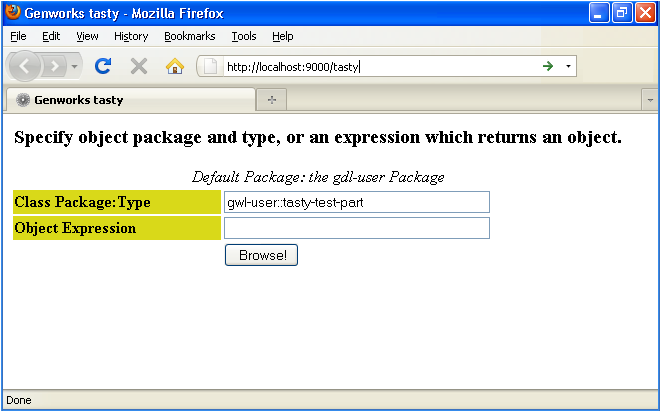
\includegraphics{../images/tasty-start.png}
\end{center}

\caption{Tasty start-up}

\label{fig:tasty-startup}

\end{figure}


Note that if the \texttt{assembly} symbol had not been exported from the \texttt{:shock-absorber} package, then a double-colon would have been needed: \texttt{shock-absorber::assembly}\footnote{use of a double-colon indicates dubious coding
practice, because it means that the code in quesion is accessing the
``internals'' or ``guts'' of another package, which may not have been
the intent of that other package's designer.}



After you specify the class package and the object type and press the
``browse'' button, the browser will bring up the utility interface
with an instance of the specified type (see figure 
\ref{fig:tastyshockabsorberpre}.



The utility interface by default is composed of three toolbars and
three view frames (tree frame, inspector frame and viewport frame
``graphical view port'').


\begin{figure}
\begin{center}
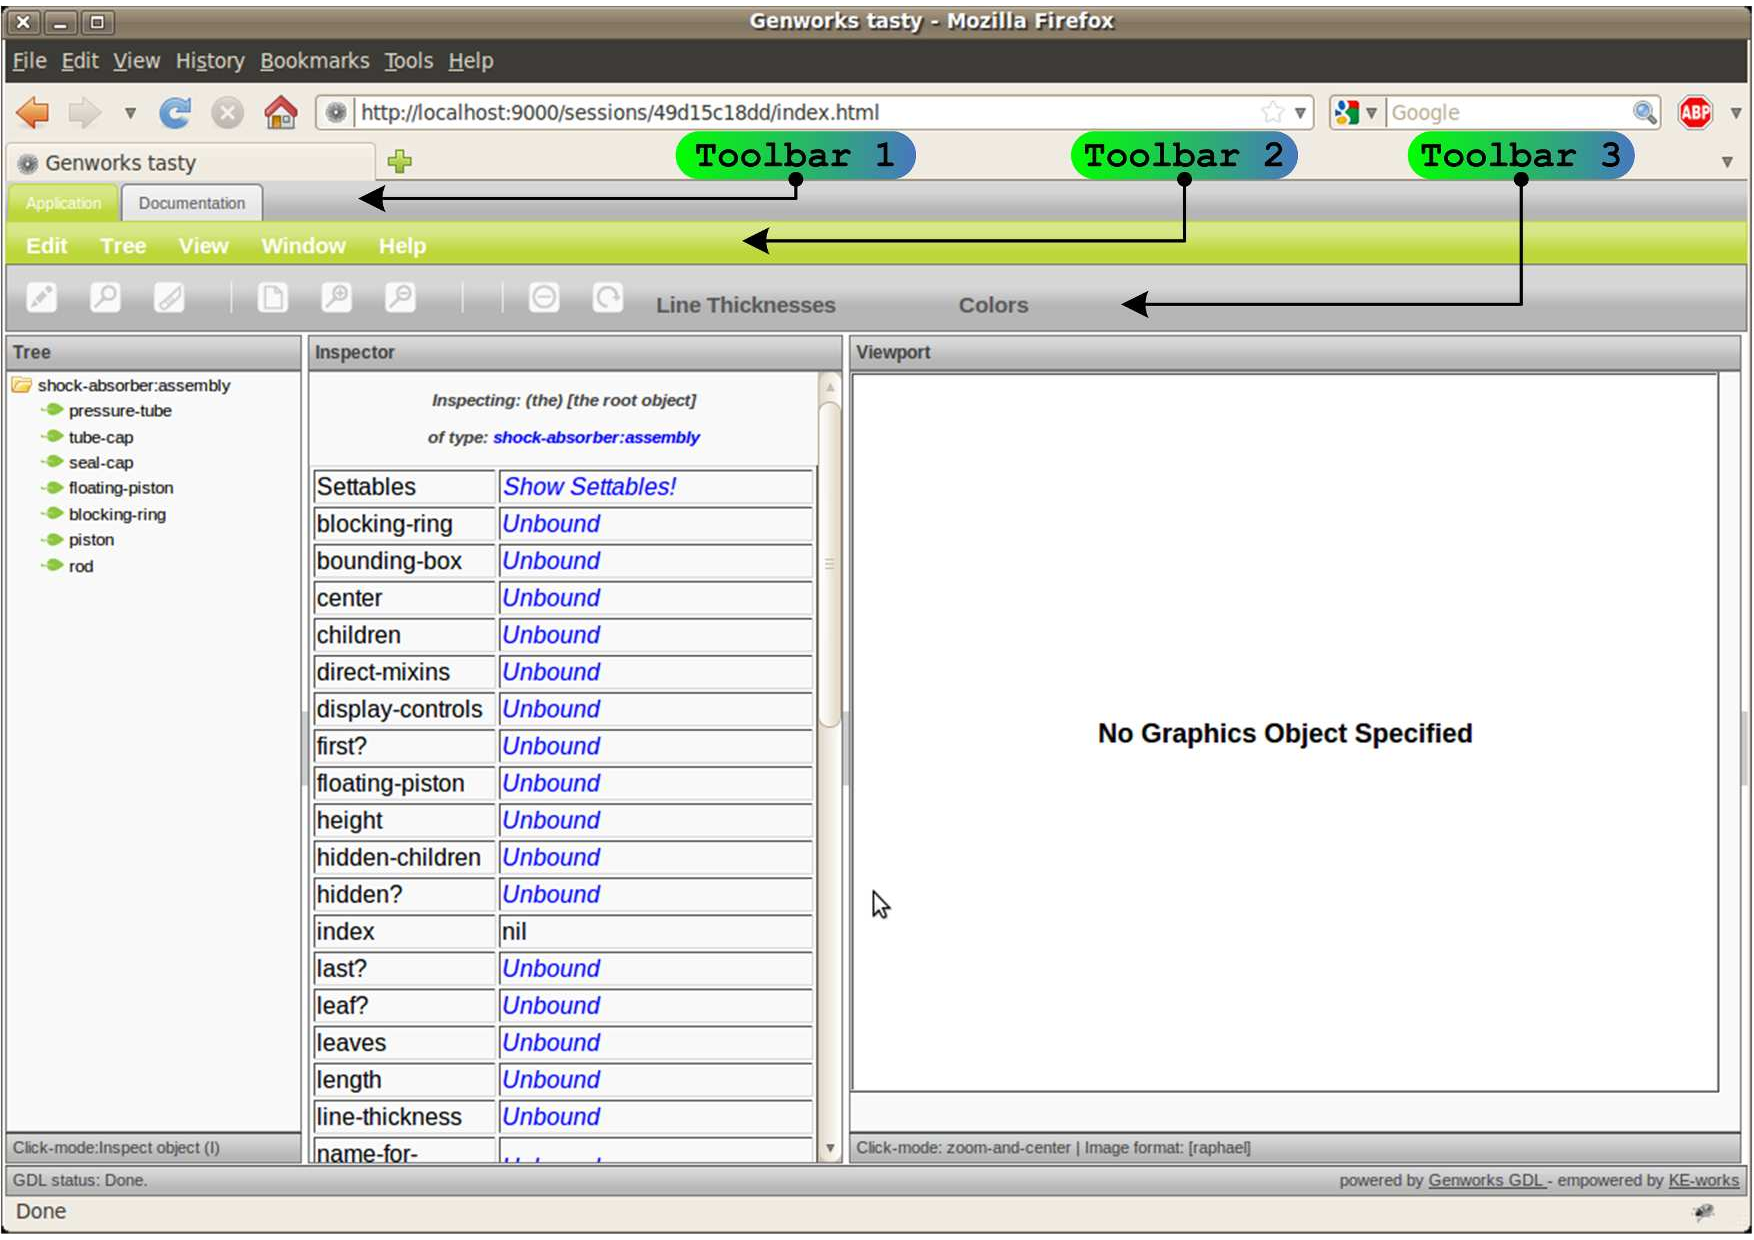
\includegraphics[width=4in,height=4in]{../images/tasty-shock-absorber-pre.pdf}
\end{center}

\caption{Tasty Interface}

\label{fig:tastyshockabsorberpre}

\end{figure}


\subsection{The Toolbars}

\label{subsec:thetoolbars}



The first toolbar consists of two ``tabs'' which allow the
user to select between the display of the application itself or the
GenDL reference documentation.



The second toolbar is designed to select various ``click modes'' for
objects and graphical viewing, and to customize the interface in other
ways. It hosts five menus: edit, tree, view, windows and
help\footnote{A File menu will be added in a future release, to
facilitate saving and restoring of instance ``snapshots'' --- at
present, this can be done programmatically.}.



The \emph{tree menu} allows the user to customize the ``click mode'' of the
mouse (or ``tap mode'' for other pointing device) for objects in the
tree, inspector, or viewport frames. The behavior follows the \emph{select-and-match} paradigm -- you first \emph{select} a mode of operation with one of the buttons or menu items, 
then \emph{match} that mode to any object in the tree frame or inspector frame by
left-clicking (or tapping). These modes are as follows:



\begin{itemize}

\item Tree: Graphical modes

\begin{description}

\item [Add Node (AN)]
Node in graphics viewport

\item [Add Leaves (AL)]
Add Leaves in graphics viewport

\item [Add Leaves indiv. (AL*)]
Add Leaves individually (so they can be deleted individually).

\item [Draw Node (DN)]
Draw Node in graphics view port (replacing any existing).

\item [Draw Leaves (DL)]
Draw Leaves in graphics view port (replacing any existing).

\item [Clear Leaves (DL)]
Delete Leaves

\end{description}



\item Tree: Inspect \& debug modes

\begin{description}

\item [Inspect object (I)]
Inspect (make the inspector frame to show the selected object).

\item [Set self to Object (B)]
Sets a global \texttt{self} variable to the selected object, so you can interact by sending messages to the object at the command prompt e.g. by typing \texttt{(the length)} or \texttt{(the children)}.

\item [Set Root to Object (SR)]
Set displayed root in Tasty tree to selected object.

\item [Up Root (UR!)]
Set displayed root in Tasty tree up one level (this is grayed out if already on root).

\item [Reset Root (RR!)]
Reset displayed root in Tasty to to the true root of the tree (this is grayed out if already on root).

\end{description}



\item Tree: frame navigation modes

\begin{description}

\item [Expand to Leaves (L)]
Nodes expand to their deepest leaves when clicked. 

\item [Expand to Children (C)]
Nodes expand to their direct children when clicked.

\item [Auto Close (A)]
When any node is clicked to expand, all other nodes close automatically.

\item [Remember State (R)]
Nodes expand to their previously expanded state when clicked.

\end{description}



\item View: Viewport Actions

\begin{description}

\item [Fit to Window!]
Fits to the graphics viewport size the displayed objects (use after a Zoom)

\item [Clear View! (CL!)]
Clear all the objects displayed in the graphics viewport.

\end{description}



\item View: Image Format

\begin{description}

\item [PNG]
Sets the displayed format in the graphics viewport to PNG (raster image with 
        isoparametric curves for surfaces and brep faces).

\item [JPEG]
Sets the displayed format in the graphics viewport to JPEG
         (raster image with isoparametric curves for surfaces and brep faces).

\item [VRML/X3D]
Sets the displayed format in the graphics viewport to
             VRML with default lighting and viewpoint (these can be changed
             programmatically). This requires a compatible plugin such as BS Contact

\item [X3DOM]
This experimental mode sets the displayed format in the graphics viewport to use the x3dom.js Javascript library,
which attempts to render X3D format directly in-browser without the need for plugins. This works best in WebGL-enabled
browsers such as a recent version of Google Chrome\footnote{Currently, it is necessary to ``Reload'' or
	   ``Refresh'' the browser window to display the geometry in
	   this mode.}.

\item [SVG/VML]
Sets the displayed format in the graphics viewport to SVG/VML\footnote{For complex objects with many display curves,
            SVG/VML can overwhelm the JavaScript engine in the web
            browser. Use PNG for these cases.}, which is a vector graphics image format displaying 
            isoparametric curves for surfaces and brep faces.

\end{description}



\item View: Click Modes

\begin{description}

\item [Zoom in]
Sets the mouse left-click in the graphics viewport to zoom in.

\item [Zoom out]
Sets the mouse left-click in the graphics viewport to zoom out.

\item [Measure distance]
Calculates the distance between two selected points from the graphics viewport.

\item [Get coordinates]
Displays the coordinates of the selected point from the graphics viewport.

\item [Select Object]
Allows the user to select an object from the graphics
                  viewport (currently works for displayed curves and
                  in SVG/VML mode only).

\end{description}



\item View: Perspective

\begin{description}

\item [Trimetric]
Sets the displayed perspective in the graphics viewport to trimetric.

\item [Front]
Sets the displayed perspective in the graphics viewport to Front (negative Y axis).

\item [Rear]
Sets the displayed perspective in the graphics viewport to Rear (positive Y axis).

\item [Left]
Sets the displayed perspective in the graphics viewport to Left (negative X axis).

\item [Right]
Sets the displayed perspective in the graphics viewport to Right (positive X axis).

\item [Top]
Sets the displayed perspective in the graphics viewport to Top (positive Z axis).

\item [Bottom]
Sets the displayed perspective in the graphics viewport to Bottom (negative Z axis).

\end{description}



\end{itemize}



The third toolbar hosts the most frequently used buttons. This
buttons have tooltips which will pop up when you hover the mouse over
them. However, these buttons are found in the second toolbar too,
except line thickness and color buttons. The line thickness and color
buttons\footnote{the design of the line thickness and color buttons is
being refined and may appear different in your installation.} expand and contract when clicked on and allows the user to
select a desired line thickness and color for the objects displayed in
the graphics viewport.



\subsection{View Frames}

\label{subsec:viewframes}



The \emph{tree frame} is a hierarchical representation of your defined
object. For example for the shock-absorber assembly this will be as
depicted in figure 
\ref{fig:tree-shock-absorber}



To draw the graphics (geometry) for the shock-absorber
leaf-level objects, you can select the ``Add Leaves (AL)'' item from
the Tree menu, then click the desired leaf to be displayed from the
tree. Alternatively, you can select the ``rapid'' button from third
toolbar which is symbolized by a pencil icon. Because this
operation (draw leaves) is frequently used, this operation is directly
available as a tooltip which will pop up when you hover the mouse over
any leaf or node in the tree.



The ``on the fly'' feature is available also for ``inspect
object,'' as the second icon when you hover the mouse over a leaf or
node.



The ``inspector'' frame allows the user to inspect (and in
some cases modify) the object instance being inspected.



For example, let's make the \texttt{piston-radius} of the shock-absorber ``settable,'' by adding the keyword \texttt{:settable}after its default expression (please review Chapter 
\ref{chap:advancedgendl} if you are not familiar or need a refresher on this GenDL
syntax). We will also pass the piston-radius down into the child \texttt{piston} object, rather than using a hard-coded value of 12 as
previously. The new assembly definition is now:
\begin{figure}
\begin{lrbox}{\boxedverb}
\begin{minipage}{\linewidth}
{\small

\begin{verbatim}
 (in-package :shock-absorber)

 (define-object  assembly (base-object)
   :input-slots ((piston-radius 12 :settable)) ;;;----modification ;
   :computed-slots ()
   :objects 
   ((pressure-tube :type 'cone
		   :center (make-point 0 70 0)
		   :length 120
		   :radius-1 13
		   :inner-radius-1 12
		   :radius-2 13
		   :inner-radius-2 12)
   
    (tube-cap :type 'cone
	      :center (make-point 0 5 0)
	      :length 10
	      :radius-1 5
	      :inner-radius-1 0
	      :radius-2 13
	      :inner-radius-2 0)

    (seal-cap :type 'cone
	      :center (make-point 0 135 0)
	      :length 10
	      :radius-1 13
	      :inner-radius-1 2.5
	      :radius-2 5
	      :inner-radius-2 2.5)
   
    (floating-piston :type 'cylinder
		     :center (make-point 0 35 0)
		     :radius 12
		     :length 10)

    (blocking-ring :type 'cone
		   :center (make-point 0 42.5 0)
		   :length 5
		   :radius-1 12
		   :inner-radius-1 10
		   :radius-2 12
		   :inner-radius-2 10)
   
    (piston :type 'cylinder
	    :center (make-point 0 125 0)
	    :radius (the piston-radius) ;;;----modification ;
	    :length 10)
   
    (rod :type 'cylinder
	 :center (make-point 0 175 0)
	 :radius 2.5
	 :length 90))
\end{verbatim}}
\end{minipage}
\end{lrbox}
\fbox{\usebox{\boxedverb}}

\caption{Shock Absorber Assembly V0.1}

\label{fig:shockabsorberassemblyv01}

\end{figure}




In this new version ``V0.1'' of the assembly, the piston radius is a
settable slot, and its value can be modified (i.e. ``bashed'') as
desired, either programmatically from the command-line, in an end-user
application, or from the Tasty environment.


\begin{figure}
\begin{center}
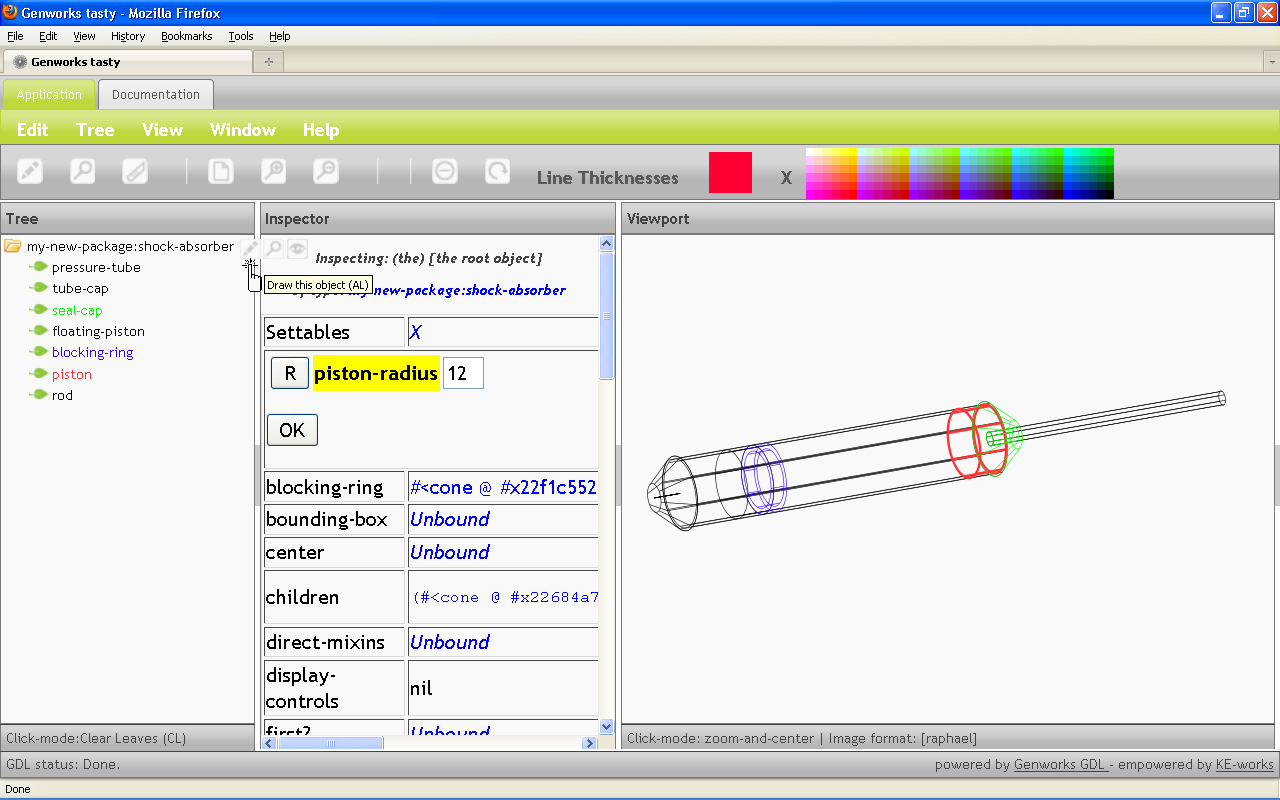
\includegraphics[width=4in,height=3in]{../images/tasty-inspector.png}
\end{center}

\caption{Tasty Inspector}

\label{fig:tasty-inspector}

\end{figure}

\begin{figure}
\begin{center}
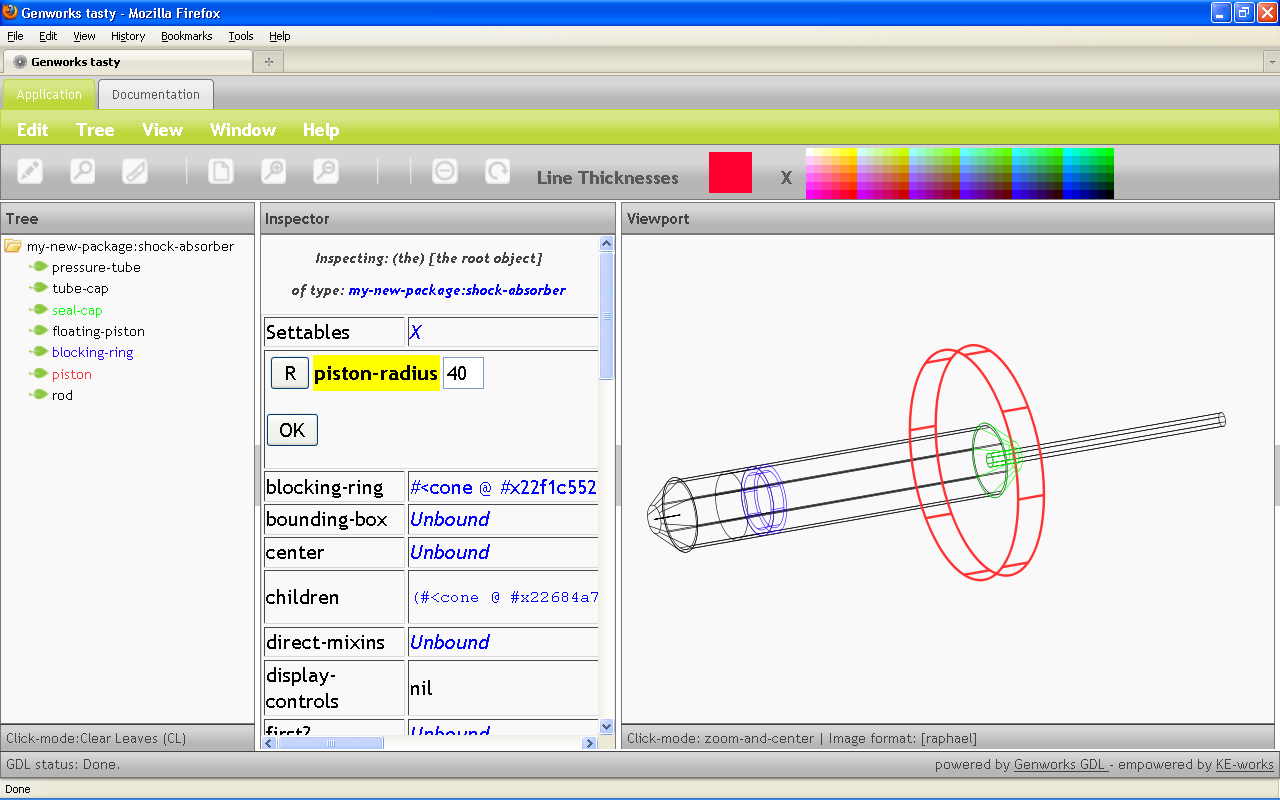
\includegraphics[width=4in,height=3in]{../images/tasty-s-slots.png}
\end{center}

\caption{Settable Slots in Tasty}

\label{fig:tasty-s-slots}

\end{figure}


To modify the value in Tasty: select ``Inspect'' mode from the Tree
menu, then select the root of the \texttt{assembly} tree to set the inspector on that object (see Figure 
\ref{fig:tasty-inspector}). Once the inspector is displaying this object, it is
possible to expand its settable slots by clicking on the ``Show
Settables!''  link. (use the ``X'' link to collapse the settable slots
view). When the settable slots area is open, the user may set the
values as desired by inputting the new value and pressing the OK
button (see Figure 
\ref{fig:tasty-s-slots}).



\chapter{Working with Geometry in Gendl}

\label{chap:workingwithgeometryingendl}



\chapter{Custom User Interfaces in GenDL}

\label{chap:customuserinterfacesingendl}



One of the strengths of GenDL is the ability to create custom
web-based user interfaces. GenDL contains a built-in web server and
supports the creation of generative \emph{web-based} user interfaces\footnote{GenDL does not contain support for native desktop
GUI applications. Although the host Common Lisp
environment (e.g. Allegro CL or LispWorks) may contain a GUI builder
and Integrated Development Environment, and you are free to use these,
GenDL does not provide specific support for them.}. Using the same \texttt{define-object} syntax which you have already learned, you can define web
pages, sections of web pages, and \emph{form control} elements such as type-in fields, checkboxes, and choice
lists. Using this capability does require a basic working knowledge of
the HTML language\footnote{We will not cover HTML in this manual, but
plentiful resources are available online and in print.}.



Any web extensions such as custom JavaScript and JavaScript libraries
can also be used, as with any standard web application.



With the primitive objects and functions in its \texttt{:gwl} package, GenDL supports both the traditional ``Web 1.0''
interfaces (with fillout forms, page submittal, and complete page
refresh) as well as so-called ``Web 2.0'' interaction with AJAX.



\section{Package and Environment for Web Development}

\label{sec:packageandenvironmentforwebdevelopment}



Similarly to \texttt{gdl:define-package}, you can use \texttt{gwl:define-package} in order to create a working package which has
access to the symbols you will need for building a web application (in
addition to all the other GenDL symbols).



The \texttt{:gwl-user} package is pre-defined and may be used for practice
work. For real projects, you should define your own package using \texttt{gwl:define-package}.



The acronym ``GWL'' stands for Generative Web Language, which is not
actually a separate language from GenDL itself, but rather a set of
primitive objects and functions available with GenDL for building web
applications. The YADD reference documentation for package
``Generative Web Language'' provides detailed specifications for all
the primitive objects and functions.



\section{Traditional Web Pages and Applications}

\label{sec:traditionalwebpagesandapplications}



To make a GenDL object presentable as a web page, the following two
steps are needed:

\begin{enumerate}

\item Mix \texttt{base-html-sheet} into the object definition.

\item define a GenDL function called \texttt{main-sheet} within the object definition.

\end{enumerate}

The \texttt{main-sheet} function should return valid
HTML for the page. The easiest way to produce HTML is with the use of
an HTML generating library, such as \href{http://weitz.de/cl-who}{CL-WHO} or \href{http://www.franz.com/support/documentation/current/doc/aserve/htmlgen.html}{HTMLGen}, both of which are built into GenDL.



For our examples we will use cl-who, which is currently the
standard default HTML generating library used internally by
GenDL. Here we will make note of the major features of cl-who while
introducing the examples; for complete documentation on cl-who, please
visit the page at Edi Weitz' website listed above.



\subsection{A Simple Static Page Example}

\label{subsec:asimplestaticpageexample}



In Figure 
\ref{fig:gwl-1}, GWL convenience macro \texttt{with-cl-who} is used; this sets up a standard default environment for outputting HTML 
within a GWL application.
\begin{figure}
\begin{lrbox}{\boxedverb}
\begin{minipage}{\linewidth}
\tiny{

\begin{verbatim}(in-package :gwl-user)

(define-object president (base-html-sheet)
  :input-slots
  ((name "Carter") (term 1976) (table-border 1))

  :functions
  ((write-html-sheet
    () (with-cl-who (:indent t)
         (:html (:head (:title (fmt "Info on President: ~a" 
                                    (the name))))
                (:body ((:table :border (the table-border))
                        (:tr (:th "Name") (:th "Term"))
                        (:tr (:td (str (the name))) 
                             (:td (str (the term)))))))))))
;;
;; Access the above example with 
;; http://localhost:9000/make?object=gwl-user::president
;;

\end{verbatim}}
\end{minipage}
\end{lrbox}
\fbox{\usebox{\boxedverb}}

\caption{Simple Static Page Example}

\label{fig:gwl-1}

\end{figure}




The code in Figure 
\ref{fig:gwl-1} produces HTML output as shown in Figure 
\ref{fig:gwl-1-html} which looks similar to Figure 
\ref{fig:gwl-1-image} in a web browser.
\begin{figure}
\begin{lrbox}{\boxedverb}
\begin{minipage}{\linewidth}
\tiny{

\begin{verbatim}
<html>
  <head>
    <title>Info on President: Carter
    </title>
  </head>
  <body>
    <table border="1">
      <tr> <th>Name</th>
           <th>Term</th>
      </tr>
      <tr> <td>Carter</td>
           <td>1976</td>
      </tr>
    </table>
  </body></html>

\end{verbatim}}
\end{minipage}
\end{lrbox}
\fbox{\usebox{\boxedverb}}

\caption{Simple Static Page Example}

\label{fig:gwl-1-html}

\end{figure}

\begin{figure}
\begin{center}
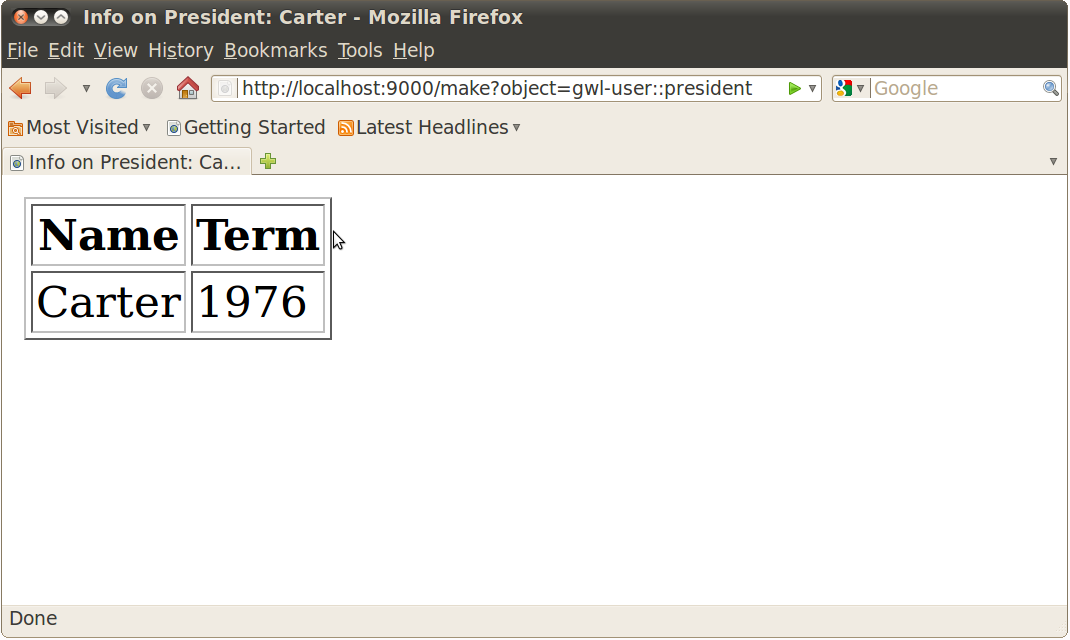
\includegraphics[width=4in,height=3in]{../images/gwl-1.png}
\end{center}

\caption{Simple Static Page Example}

\label{fig:gwl-1-image}

\end{figure}




Several important concepts are packed into this example. Note the following:

\begin{itemize}

\item Our convenience macro \texttt{with-cl-who} is used to wrap the native \texttt{with-html-output} macro which comes with the cl-who library.

\item We use the keyword argument \texttt{:indent t} in order to pretty-print the generated HTML. This does
     not affect the browser display but can make the generated HTML
     easier to read and debug. This option should be left as nil (the
     default) for production deployments.

\item The \texttt{fmt} symbol has special meaning
      within the cl-who environment and works the same as a Common
      Lisp \texttt{format nil}in order to evaluate a format
      string together with matching arguments, and produce a string at
      runtime.

\item The \texttt{str} symbol has special meaning
      within the cl-who environment and works by evaluating an
      expression at runtime to return a string or other printable
      object, which is then included at that point in the HTML output.

\item Expressions within the \texttt{body} of an
      HTML tag have to be evaluated, usually by use of the \texttt{fmt} or \texttt{str} in cl-who.  There are three examples of this in the
      above sample: one \texttt{fmt} and two \texttt{str}.

\item Expressions within a \emph{tag attribute} are always evaluated automatically, and so do 
\textbf{not} require a \texttt{str} or other special symbol to force evaluation at
      runtime. Tag attributes in HTML (or XML) are represented as a
      plist spliced in after a tag name, wrapped in extra parentheses
      around the tag name. In the sample above, the \texttt{:border (the table-border)} is an example of a tag attribute on the \texttt{:table} tag. Notice that the expression \texttt{(the table-border)} does not need \texttt{str} in order to be evaluated - it gets evaluated automatically.

\item In cl-who, if a tag attribute evaluates to \texttt{nil}, then that tag attribute will be left out of the output
      completely. For example if \texttt{(the table-border)} evaluates to nil, then the \texttt{:table} tag will be outputted without any attributes at
      all. This is a convenient way to conditionalize tag
      attributes.

\item The URL \texttt{http://localhost:9000/make?object=gwl-user::president} is published automatically based on the package and
      name of the object definition. When you visit this URL, the
      response is redirected to a unique URL identified by
      a \emph{session ID}. This ensures that each user to your
      application site will see their own specific instance of the
      page object. The session ID is constructed from a combination of
      the current date and time, along with a pseudo-random
      number.

\end{itemize}





\subsection{A Simple Dynamic Page which Mixes HTML and Common Lisp/GenDL}

\label{subsec:asimpledynamicpagewhichmixeshtmlandcommonlisp/gendl}



Within the cl-who environment, it is possible to include any standard
Common Lisp structures such as \texttt{let}, \texttt{dolist} , \texttt{dotimes}, etc, which accept a \emph{body} of code. The requirement is that any internal code body
	  must be wrapped in a list beginning with the special symbol \texttt{htm}, which has meaning to cl-who. 


\begin{figure}
\begin{lrbox}{\boxedverb}
\begin{minipage}{\linewidth}
\tiny{

\begin{verbatim}(in-package :gwl-user)

(define-object presidents (base-html-sheet)
  :input-slots
  ((presidents (list (list :name "Ford"
                           :term 1974)
                     (list :name "Carter"
                           :term 1976)
                     (list :name "Clinton"
                           :term 1992)
                     (list :name "Bush"
                           :term 2000)
                     (list :name "Obama"
                           :term 2008)))
   
   (table-border 1))

  :functions
  ((write-html-sheet
    () 
    (with-cl-who (:indent t)
      (let ((title (format nil "Info on ~a Presidents:" 
                           (length (the presidents)))))
        (htm
         (:html 
          (:head (:title (str title)))
          (:body 
           (:p (:c (:h3 (str title))))
           ((:table :border (the table-border))
            (:tr (:th "Name") (:th "Term"))
            (dolist (president (the presidents))
              (htm      
               (:tr (:td (str (getf president :name)))
                    (:td (str (getf president :term)))))))))))))))
;;
;; Access the above example with 
;; http://localhost:9000/make?object=gwl-user::presidents
;;

\end{verbatim}}
\end{minipage}
\end{lrbox}
\fbox{\usebox{\boxedverb}}

\caption{Mixing Static HTML and Dynamic Content}

\label{fig:gwl-2}

\end{figure}

\begin{figure}
\begin{center}
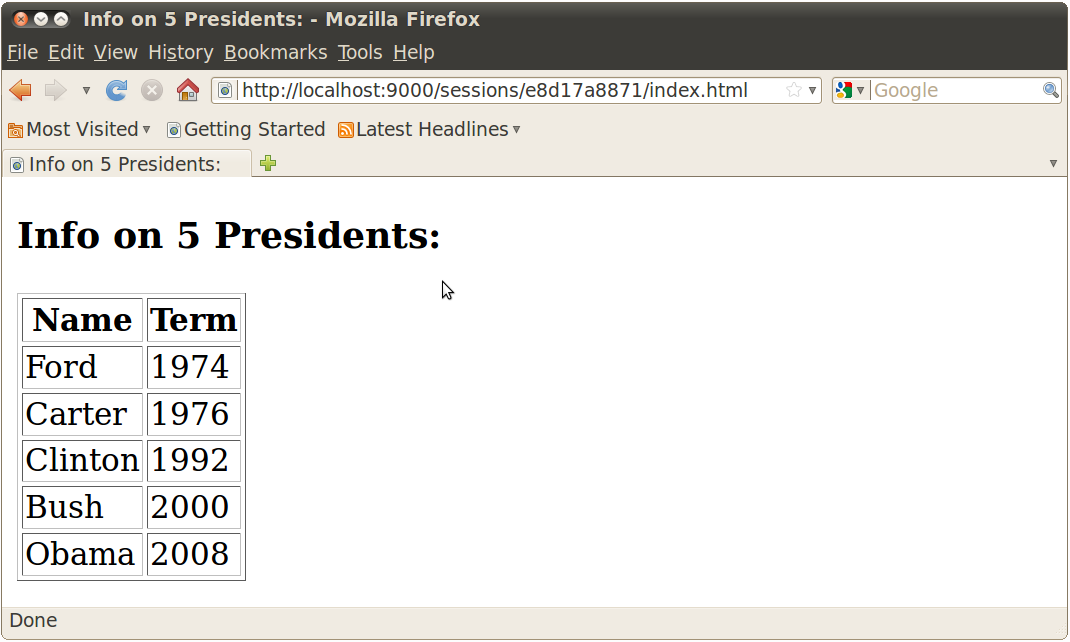
\includegraphics[width=4in,height=3in]{../images/gwl-2.png}
\end{center}

\caption{Mixing Static HTML and Dynamic Content}

\label{fig:gwl-2-image}

\end{figure}


The example in Figure 
\ref{fig:gwl-2}  uses this technique to output an HTML table row for each ``row'' of data in a list of lists.
The output looks similar to Figure 
\ref{fig:gwl-2-image} in a web browser.



Note the following from this example:

\begin{itemize}

\item \texttt{title} is a \texttt{let} variable, so we use \texttt{(str title)} to evaluate it as a string. We do not use \texttt{(str (the title))} because \texttt{title} is a local variable and not a message (i.e. slot) in the object.

\item Inside the \texttt{dolist}, we ``drop back into'' HTML mode using the \texttt{htm} operator.

\end{itemize}





\subsection{Linking to Multiple Pages}

\label{subsec:linkingtomultiplepages}



The base-html-sheet mixin provides a \texttt{self-link} message for the purpose of generating a hyperlink to that
page. Typically you will have a ``parent'' page object which links to
its ``child'' pages, but GenDL pages can link to other pages anywhere
in the GenDL tree\footnote{In order for dependency-tracking to work
properly, the pages must all belong to the same tree, i.e. they must
share a common root object.}.
\begin{figure}
\begin{lrbox}{\boxedverb}
\begin{minipage}{\linewidth}
\tiny{

\begin{verbatim}(in-package :gwl-user)

(define-object presidents-with-pages (base-html-sheet)
  :input-slots
  ((presidents (list (list :name "Ford" :term 1974)
                     (list :name "Carter" :term 1976)
                     (list :name "Clinton" :term 1992)
                     (list :name "Bush" :term 2000)
                     (list :name "Obama" :term 2008)))
   
   (table-border 1))
  
  
  :objects
  ((president-pages :type 'president-page
                    :sequence (:size (length (the presidents)))
                    :name (getf (nth (the-child index) (the presidents))
                                :name)
                    :term (getf (nth (the-child index) (the presidents))
                                :term)))


  :functions
  ((write-html-sheet
    () 
    (with-cl-who (:indent t)
      (let ((title (format nil "Info on ~a Presidents:" 
                           (length (the presidents)))))
        (htm
         (:html 
          (:head (:title (str title)))
          (:body 
           (:p (:c (:h3 (str title))))
           (:ol
            (dolist (page (list-elements (the president-pages)))
              (htm      
               (:li
                (the-object 
                 page 
                 (write-self-link :display-string 
                                  (the-object page name)))))))))))))))

;;
;; Access the above example with 
;; http://localhost:9000/make?object=gwl-user::presidents-with-pages
;;

\end{verbatim}}
\end{minipage}
\end{lrbox}
\fbox{\usebox{\boxedverb}}

\caption{Linking to Multiple Pages}

\label{fig:gwl-3}

\end{figure}

\begin{figure}
\begin{lrbox}{\boxedverb}
\begin{minipage}{\linewidth}
\tiny{

\begin{verbatim}(in-package :gwl-user)

(define-object president-page (base-html-sheet)
  :input-slots
  (name term)
  
  :functions
  ((write-html-sheet
    ()
    (with-cl-who ()
      (let ((title (format nil "Term for President ~a:" 
                           (the name))))
        (htm
         (:html 
          (:head (:title (str title)))
          (:body 
           (the (write-back-link :display-string "&lt;Back"))
           (:p (:c (:h3 (str title))))
           (:p (str (the term)))))))))))

      

\end{verbatim}}
\end{minipage}
\end{lrbox}
\fbox{\usebox{\boxedverb}}

\caption{Linking to Multiple Pages}

\label{fig:gwl-3a}

\end{figure}
 In Figures 
\ref{fig:gwl-3} and 
\ref{fig:gwl-3a}, we provide links from a parent page into a child page
with detailed information on each president. The output looks similar
to Figure 
\ref{fig:gwl-3-image} in a web browser.
\begin{figure}
\begin{center}
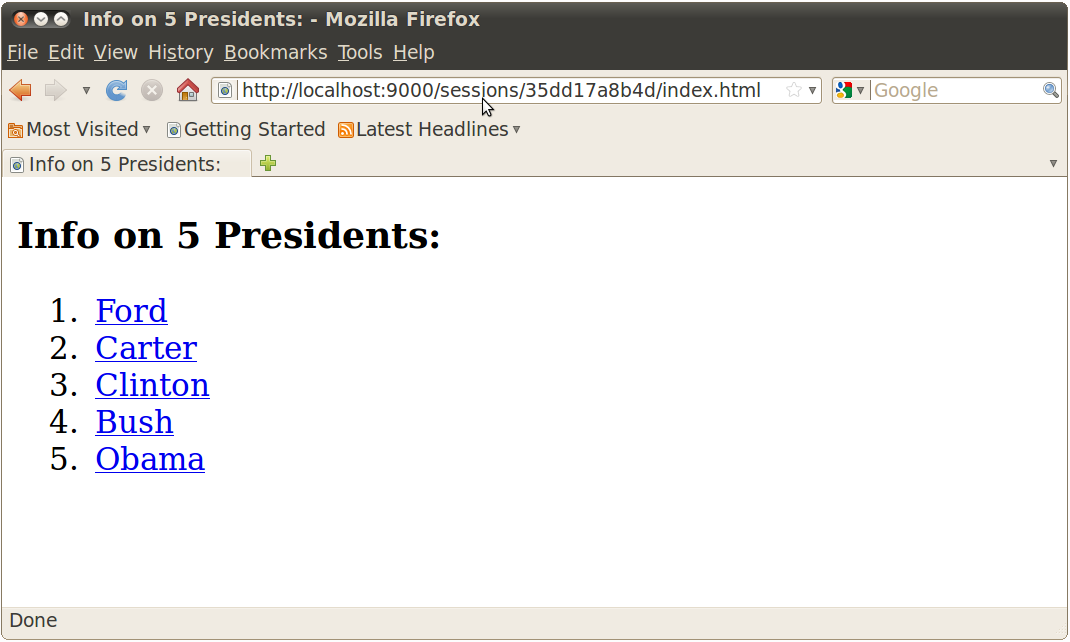
\includegraphics[width=4in,height=3in]{../images/gwl-3.png}
\end{center}

\caption{Linking to Multiple Pages}

\label{fig:gwl-3-image}

\end{figure}




 Note the following from this example:

\begin{itemize}

\item The \texttt{write-self-link} message is a function which can take a keyword argument
   of \texttt{:display-string}. This string is used for the actual hyperlink text.

\item There is a \texttt{write-back-link} message which similarly can take a keyword argument of \texttt{:display-string}. This generates a link back to \texttt{(the return-object)} which, by default in base-html-sheet, is \texttt{(the parent).}

\end{itemize}





\subsection{Form Controls and Fillout-Forms}

\label{subsec:formcontrolsandfillout-forms}



\subsubsection{Form Controls}

\label{subsubsec:formcontrols}



GenDL provides a set of primitives useful for generating
            the standard HTML
            form-controls@footnote{http://www.w3.org/TR/html401/interact/forms.html}
            such as text, checkbox, radio, submit, menu, etc. These
            should be instantiated as child objects in the page, then
            included in the HTML for the page
            using \texttt{str} within an
            HTML \texttt{form} tag (see next section).



\subsubsection{Fillout Forms}

\label{subsubsec:filloutforms}



A traditional web application must enclose form controls inside a \texttt{form} tag and specify an \texttt{action} (a web URL) to receive and respond to the 
form submission. The response will cause the entire page to refresh with
a new page. In GenDL, such a form can be generated by wrapping the layout
of the form controls within the \texttt{with-html-form} macro.


\begin{figure}
\begin{lrbox}{\boxedverb}
\begin{minipage}{\linewidth}
\tiny{

\begin{verbatim}(in-package :gwl-user)

(define-object revenue-lookup-old-school (base-ajax-sheet)
  
  :input-slots
  
  ((revenue-data '(2003 25000
                   2004 34000
                   2005 21000
                   2006 37000
                   2007 48000
                   2008 54000
                   2009 78000)))
  
  :functions
  
  ((write-html-sheet
    ()
    (with-cl-who ()
      (when *developing?* (str (the development-links)))
      (with-html-form (:cl-who? t)
        (:p (str (the table-border html-string)))
        (:p (str (the cell-padding html-string)))
        (:p (str (the selected-year html-string)))
        (:p ((:input :type :submit :value " OK "))))
      (:p ((:table :border (the table-border value)
                   :cellpadding (the cell-padding value))
           (:tr (:th (fmt "Revenue for Year ~a:" 
                          (the selected-year value)))
                (:td (str (getf (the revenue-data) 
                                (the selected-year value))))))))))

  :objects
  
  ((table-border :type 'menu-form-control
                 :size 1 :choice-list '(0 1)
                 :default 0)
   
   (cell-padding :type 'menu-form-control
                 :size 1 :choice-list '(0 3 6 9 12)
                 :default 0)
   
   (selected-year :type 'menu-form-control
                  :size 1 :choice-list (plist-keys (the revenue-data))
                  :default (first (the-child choice-list)))))
   

(publish-gwl-app "/revenue-lookup-old-school" 
                 "gwl-user::revenue-lookup-old-school")


;;
;; Access the above example with 
;; http://localhost:9000/make?object=gwl-user::revenue-lookup-old-school
;;

\end{verbatim}}
\end{minipage}
\end{lrbox}
\fbox{\usebox{\boxedverb}}

\caption{Form Controls and Fillout Forms}

\label{fig:gwl-3b}

\end{figure}

\begin{figure}
\begin{center}
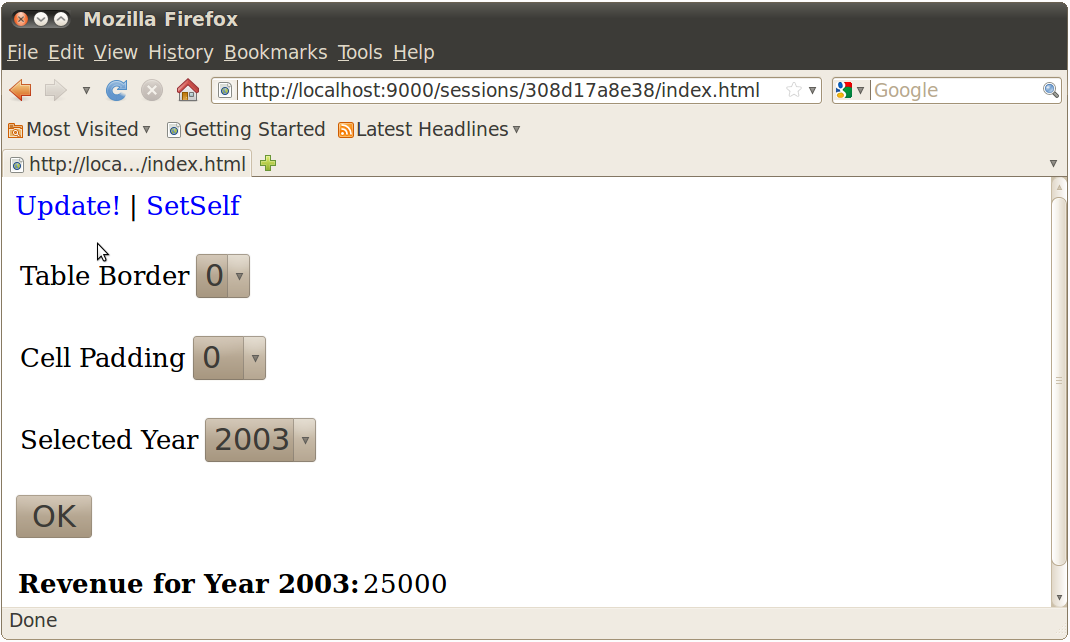
\includegraphics[width=4in,height=3in]{../images/gwl-3b.png}
\end{center}

\caption{Form Controls and Fillout Forms}

\label{fig:gwl-3b-image}

\end{figure}


In Figure 
\ref{fig:gwl-3b} is an example which allows the user to enter a year, and the 
application will respond with the revenue amount for that year. Additional
form controls are also provided to adjust the table border and cell padding.



This example, when instantiated in a web browser, might look as shown in Figure 
\ref{fig:gwl-3b-image}.



\section{Partial Page Updates with gdlAjax}

\label{sec:partialpageupdateswithgdlajax}



AJAX stands for Asynchronous JavaScript and
XML \footnote{http://en.wikipedia.org/wiki/Ajax\_(programming)}, and allows for more interactive web applications which
respond to user events by updating only part of the web page. The
``Asynchronous'' in Ajax refers to the ability for a web page to
continue interacting while one part of the page is being updated by a
server response. Requests need not be Asynchronous, they can also be
Synchronous (``SJAX''), which would cause the web browser to block
execution of any other tasks while the request is being carried
out. The ``XML'' refers to the format of the data that is typically
returned from an AJAX request.



GenDL contains a simple framework referred to as \emph{gdlAjax} which supports a uniquely convenient and generative
approach to AJAX (and SJAX). With gdlAjax, you use standard GenDL
object definitions and child objects in order to model the web page
and the sections of the page, and the dependency tracking engine which
is built into GenDL automatically keeps track of which sections of the
page need to be updated after a request.



Moreover, the state of the internal GenDL model which represents the
page and the page sections is kept identical to the displayed state of
the page. This means that if the user hits the ``Refresh'' button in
the browser, the state of the page will remain unchanged. This is not
true of some other Ajax frameworks.



\subsection{Steps to Create a gdlAjax Application}

\label{subsec:stepstocreateagdlajaxapplication}



First, it is important to understand that the fundamentals from the
previous section on Standard Web Applications still apply for gdlAjax
applications --- that is, HTML generation, page linking, etc. These
techniques will all still work in a gdlAjax application.



To produce a gdlAjax application involves three main differences from
a standard web application:

\begin{enumerate}

\item You mix in \texttt{base-ajax-sheet} instead of \texttt{base-html-sheet}. \texttt{base-ajax-sheet} mixes in \texttt{base-html-sheet}, so it will still provide all the functionality of that
   mixin. In fact, you can use \texttt{base-ajax-sheet} in standard web applications and you won't notice any difference if you do
    everything else the same.

\item Instead of a \texttt{write-html-sheet} message, you specify a \texttt{main-sheet-body} message. The \texttt{main-sheet}  can be a computed-slot or GenDL function,
    and unlike the \texttt{write-html-sheet} message, it should
    simply return a string, not send output to a stream. Also, it only
    fills in the body of the page --- everything between the <body>
    and </body> tags. The head tag of the page is filled in
    automatically and can be customized in various ways.

\item Any sections of the page which you want to be able
      to change themselves in response to an Ajax call must be made
      into separate page sections, or ``sheet sections,'' and the HTML
      for their \texttt{main-div} included in the main page's \texttt{main-sheet-body}by use of cl-who's \texttt{str} directive.

\end{enumerate}


\begin{figure}
\begin{lrbox}{\boxedverb}
\begin{minipage}{\linewidth}
\tiny{

\begin{verbatim}(in-package :gwl-user)

(define-object revenue-lookup (base-ajax-sheet)
  
  :input-slots
  
  ((revenue-data '(2003 25000
                   2004 34000
                   2005 21000
                   2006 37000
                   2007 48000
                   2008 54000
                   2009 78000)))
  
  :computed-slots
  
  ((main-sheet-body 
    (with-cl-who-string ()
      (str (the main-section main-div)))))
  
  :objects
  
  ((table-border :type 'menu-form-control
                 :size 1
                 :choice-list '(0 1)
                 :default 0
                 :ajax-submit-on-change? t)
   
   (cell-padding :type 'menu-form-control
                 :size 1
                 :choice-list '(0 3 6 9 12)
                 :default 0
                 :ajax-submit-on-change? t)
   
   (selected-year :type 'menu-form-control
                  :size 1
                  :choice-list (plist-keys (the revenue-data))
                  :default (first (the-child choice-list))
                  :ajax-submit-on-change? t)
   
   (main-section 
    :type 'sheet-section
    :inner-html (with-cl-who-string ()
                 (:p (str (the development-links)))
                 (:p (str (the table-border html-string)))
                 (:p (str (the cell-padding html-string)))
                 (:p (str (the selected-year html-string)))
                 (:p ((:table :border (the table-border value)
                              :cellpadding (the cell-padding value))
                      (:tr (:th (fmt "Revenue for Year ~a:" 
                                     (the selected-year value)))
                           (:td (str (getf (the revenue-data) 
                                           (the selected-year value)))))))))))

(publish-gwl-app "/revenue-lookup" 
                 "gwl-user::revenue-lookup")





\end{verbatim}}
\end{minipage}
\end{lrbox}
\fbox{\usebox{\boxedverb}}

\caption{Partial Page Updates with GdlAjax}

\label{fig:gwl-4}

\end{figure}




Note the following from the example in Figure 
\ref{fig:gwl-4}:

\begin{itemize}

\item We mix in \texttt{base-ajax-sheet} and specify a \texttt{main-sheet-body} slot, which uses \texttt{with-cl-who-string} to compute a string
                   of HTML. This approach is also easier to debug,
                   since the \texttt{main-sheet-body} string
                   can be evaluated in the tasty inspector or at the
                   command-line.

\item We use \texttt{str} to include the string for the main page
        section (called \texttt{main-section} in this example) into the \texttt{main-sheet-body}.

\item In the \texttt{main-section}, we also
        use \texttt{str} to include the html-string for each of
        three form-controls. We have provided a form control for the
        table border, the table padding, and the revenue year to look
        up.

\item The only page section in this example is \texttt{(the main-section)}. This is defined as a child object, and has its \texttt{inner-html} computed in the parent and passed in as an input. The \texttt{sheet-section} will automatically compute a \texttt{main-div} message based on the \texttt{inner-html} that we are passing in. The \texttt{main-div} is simply the \texttt{main-view}, wrapped with
               an HTML DIV (i.e. ``division'') tag which contains a unique
               identifier for this section, derived from the root-path
               to the GenDL object in the in tree which represents the
               sheet section.

\item We introduce the CL function \texttt{gwl:publish-gwl-app}, which makes available a simplified URL for visiting an instance of this
        object in the web browser. In this case, we can access the
        instance using \texttt{http://localhost:9000/revenue-lookup}

\end{itemize}





\subsection{Including Graphics}

\label{subsec:includinggraphics}



The fundamental mixin or child type to make a graphics viewport is \texttt{base-ajax-graphics-sheet}. This object definition takes several optional input-slots, but the most essential are the \texttt{:display-list-objects} and the \texttt{:display-list-object-roots}. As indicated by their names, you specify a list of nodes to include in
the graphics output with the \texttt{:display-list-objects}, and a list of nodes whose \texttt{leaves} you want to display in the graphics output with the \texttt{:display-list-object-roots}. View controls, rendering format, action to take when clicking on objects, etc, 
can be controlled with other optional input-slots.


\begin{figure}
\begin{lrbox}{\boxedverb}
\begin{minipage}{\linewidth}
\tiny{

\begin{verbatim}(in-package :gwl-user)

(define-object box-with-inputs (base-ajax-sheet)
  
  :computed-slots
  ((use-raphael? t)
   
   (main-sheet-body 
    (with-cl-who-string ()
      (:p (when *developing?* (str (the development-links))))
      (:p (str (the inputs-section main-div)))
      (:table
       (:tr
        (dolist (viewport (list-elements (the viewport-sections)))
          (htm (:td (:td (str (the-object viewport main-div)))))))))))
  
  :objects
  ((box :type 'box
        :height (the inputs-section box-height value)
        :width (the inputs-section box-width value)
        :length (the inputs-section box-length value))
   
   (inputs-section :type 'inputs-section)

   (viewport-sections
    :type 'base-ajax-graphics-sheet
    :sequence (:size 2)
    :view-direction-default (ecase (the-child index)
                              (0 :top) (1 :trimetric))
    :image-format-default :raphael
    :display-list-objects (list (the box))
    :length 250 :width 250)))
  

 
(define-object inputs-section (sheet-section)
  
  :computed-slots
  ((inner-html (with-cl-who-string ()
                (:p (str (the box-length html-string)))
                (:p (str (the box-width html-string)))
                (:p (str (the box-height html-string))))))

  :objects 
  ((box-length :type 'text-form-control
               :default 25
               :ajax-submit-on-change? t)
   (box-width :type 'text-form-control
              :default 35
              :ajax-submit-on-change? t)
   (box-height :type 'text-form-control
               :default 45
               :ajax-submit-on-change? t)))


(publish-gwl-app "/box-with-inputs" 
                 "gwl-user::box-with-inputs")

;;
;; Access the above example with 
;; http://localhost:9000/make?object=gwl-user::box-with-inputs
;;

\end{verbatim}}
\end{minipage}
\end{lrbox}
\fbox{\usebox{\boxedverb}}

\caption{Including Graphics in a Web Page}

\label{fig:gwl-5}

\end{figure}

\begin{figure}
\begin{center}
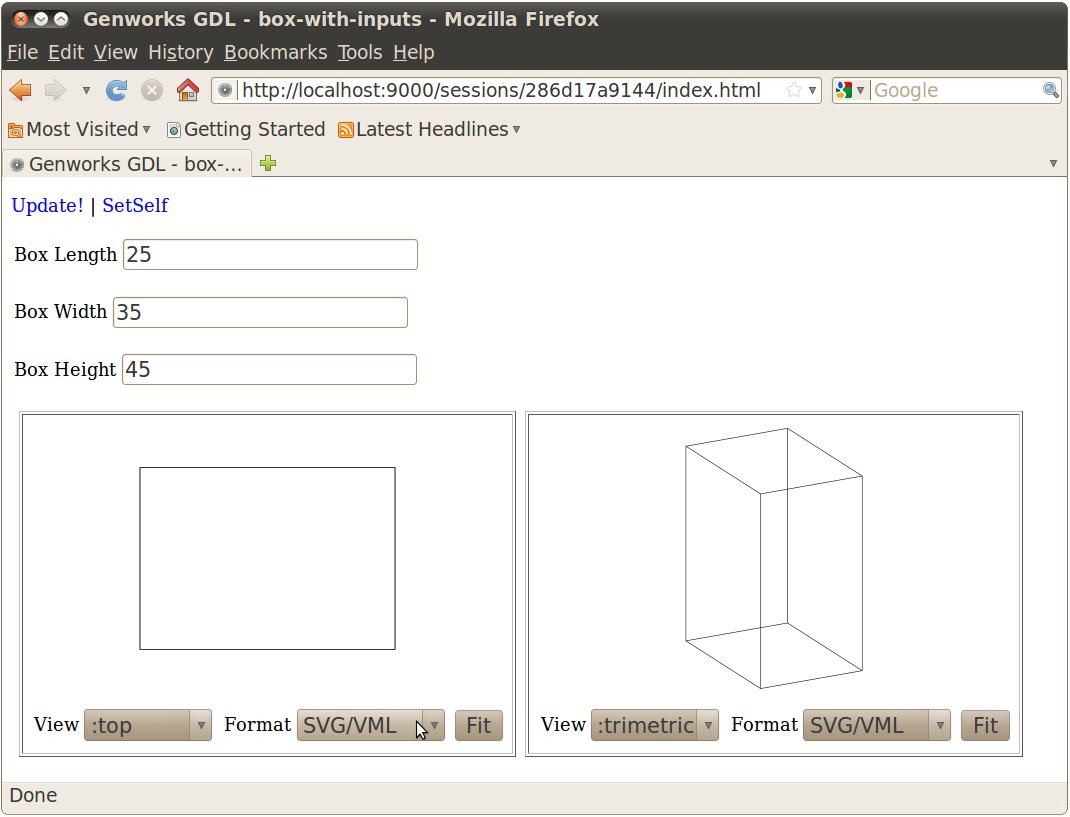
\includegraphics[width=4in,height=3in]{../images/gwl-5.png}
\end{center}

\caption{Including Graphics}

\label{fig:gwl-5-image}

\end{figure}


The example in Figure 
\ref{fig:gwl-5} contains a simple box with two graphics viewports
and ability to modify the length, height, and and with of the box:



This will produce a web browser output similar to what is shown in Figure 
\ref{fig:gwl-5-image}.



Note the following from this example:

\begin{itemize}

\item The \texttt{(:use-raphael? t)} enables raphael for SVG or VML output.

\item The \texttt{:raphael} image-format generates SVG or VML, depending on the browser.

\item We conditionally include development-links for full Update and SetSelf! actions.

\item We include two viewports in the \texttt{main-sheet-body}, elements from a sequence of size 2.

\item In the inputs-section, we use
                  the \texttt{html-string} message from each
                  form-control to display the default
                  decoration (prompt, etc).

\end{itemize}





\chapter{More Common Lisp for Gendl}

\label{chap:morecommonlispforgendl}



\chapter{Advanced Gendl}

\label{chap:advancedgendl}



\chapter*{Upgrade Notes}

\label{chap:upgradenotes}

GDL 1580 marked the end of a major branch of GDL development,
and 1581 was actually a major new version. With 1581, an open-source
version was released, and eventually the name was changed to
Gendl. 

This chapter lists the typical modifications you will want to consider
for upgrading from GDL 1580 to Gendl 1582.

\begin{itemize}

\item (update-gdl ..) is not yet available for 1582. Instead
of updating incrementally with patches, Gendl 1582 is released on a
monthly basis in conjunction with Quicklisp releases.  Updating
quicklisp involves downloading a full Genworks source code tree and
running a build script. Information on this procedure is provided in
Section 
\ref{subsec:usingquicklisp}.

\item (make-gdl-app ..) not yet available for 1582. We are
preparing the Enterprise Edition of 1582 which will include the
make-gdl-app function, which creates Runtime applications without the
compiler or Gendl development facilities.  If you are an Enterprise
licensee, are ready to release Runtime applications on 1582, and you
have not received information on the Enterprise Edition, please
contact support@genworks.com

\item (register-asdf-systems) and the \texttt{"3rdpty/"} directory are no longer needed or available. Instead, we depend on the Quicklisp
system. Details of Quicklisp are available at \href{http://www.quicklisp.org}. See Section 
\ref{subsec:usingquicklisp} for information about how to use Quicklisp with Gendl.

\item There is a system-wide gdlinit.cl in the application
       directory, and this may have some default information which
       ships with Gendl. There is a personal one in home directory,
       which you should modify if you want to customize anything.

\item Slime debugging is different from the ELI emacs debugger. The main thing to know is 
to press ``a'' or ``q'' to pop out of the current error. Full documentation for the Slime debug mode
is available with the \href{http://common-lisp.net/project/slime/doc/html/Debugger.html}{Slime documentation}.

\item color-themes -- Gendl now ships with the Emacs
       color-theme package. You can select a different color theme with \texttt{M-x color-theme-select}. Press [Enter] or middle-mouse on a color theme to apply it.

\item Gendl files can now end with \texttt{.lisp} or \texttt{.gdl}. The new \texttt{.gdl} extension will work for emacs Lisp mode and will work with
	 cl-lite, ASDF, and Quicklisp for including source files in application systems. We recommend migrating
to the new \texttt{.gdl} extension for files containing \texttt{define-object}, \texttt{define-format}, and \texttt{define-lens} forms, and any other future toplevel defining forms introduced by Gendl, in order to distinguish 
from files containing raw Common Lisp code.

\item in gdlAjax, HTML for a sheet-section is given in the slot called \texttt{inner-html} instead of \texttt{main-view}. This name change was made to clarify what exactly is
	 expected in this slot -- it is the innerHTML of the page
	 division represented by the current sheet-section. If you
	 want to make your code back-compatible with GDL 1580, you can
	 use the following form in place of old occurences of \texttt{main-view}: 

\begin{verbatim}... #+allegro-v8.1 main-view #-allegro-v8.1 inner-html ...
\end{verbatim}

\end{itemize}



\backmatter



\printindex



\end{document}

